\documentclass{anstrans}

%%%% packages and definitions (optional)
\usepackage{graphicx} % allows inclusion of graphics
\usepackage{booktabs} % nice rules (thick lines) for tables
\usepackage{microtype} % improves typography for PDF
\usepackage{xcolor} % improves typography for PDF


\newcommand{\SN}{S$_N$}
\renewcommand{\vec}[1]{\bm{#1}} % vector is bold italic
\newcommand{\vd}{\bm{\cdot}} % slightly bold vector dot
\newcommand{\grad}{\vec{\nabla}} % gradient
\newcommand{\ud}{\mathop{}\!\mathrm{d}} % upright derivative symbol

%%%% changes from the original 'anstrans' class
\usepackage{fancyhdr} % allows headers and footers

\renewcommand\headrule{} % remove underline in the header
\setcounter{secnumdepth}{1}
\renewcommand{\thesection}{\Roman{section}.}
\renewcommand{\thesubsection}{\arabic{subsection}.}
\renewcommand{\thesubsubsection}{\Alph{subsubsection}.}
\makeatletter
\renewcommand*{\@seccntformat}[1]{\csname the#1\endcsname\hspace{1mm}}
\makeatother

%%TAREK ADDITIONS%%%%%%
\newcommand{\tcr}[1]{\textcolor{red}{#1}}
%Creating a norm command
\newcommand{\norm}[1]{\left\lVert#1\right\rVert}
\newcommand{\vr}{\vec{r}}
\newcommand{\vo}{\vec{\Omega}}
%Allow page breaks within align
\allowdisplaybreaks
\usepackage{listings}
%Algorithm
\usepackage{algorithm}
\usepackage{algorithmic}
\renewcommand{\arraystretch}{1}
%%%%%%%%%%%%%%%%%%%%%%%%%%%%%%%%%%%

%%%% Header
\pagestyle{fancy}
\fancyhf{}
\fancyhead[L]{\fontsize{9}{9} \itshape
M\&C 2017 - International Conference on Mathematics \& Computational Methods Applied to Nuclear Science \& Engineering,
\\ Jeju, Korea, April 16-20, 2017, on USB (2017)
}


%%%% Maketitle
\title{An Approach for Load Balancing Massively Parallel Transport Sweeps on Unstructured Grids}
\author{Tarek H. Ghaddar, Jean C. Ragusa}

\institute{
Dept. of Nuclear Engineering, Texas A\&M University, College Station, TX, 77843-3133
}

\email{tghaddar@tamu.edu \and jean.ragusa@tamu.edu}


%%%% Abstract
\begin{document}
\vspace*{-42pt}
\begin{strip}
\centering{\parbox{153mm}{{\bf Abstract} \itshape - 
Load balancing refers to the practice of distributing approximately equal amounts of work among processors so that all processors are kept busy all of the time.
When running massively parallel codes, load balancing is a priority in order to improve parallel efficiency. 
Load balancing is important in order to minimize idle time for all processors by equally distributing (as much as possible) the work for each processor. 
Here, we discuss load-balanced problems in terms of an (approximately) equal number of degrees of freedom per processor, provided that we are employing a partitioning scheme that
minimizes idle time. 
Recently , an unstructured meshing capability was implemented in PDT, Texas A\&M University's massively parallel deterministic transport code, hence allowing the user to define more realistic problem geometries and to define 3D problems through the extrusion of 2D meshes. However, unstructured grids are significantly  harder to load balance than logically-Cartesian meshes. In this work, we propose a load balancing algorithm that is now implemented in PDT in order to minimize a specific load-imbalance metric. Several numerical test cases are provided.}}
\vspace*{14pt}
\end{strip}


%%%%%%%%%%%%%%%%%%%%%%%%%%%%%%%%%%%%%%%%%%%%%%%%%%%%%%%%%%%%%%%%%%%%%%%%%%%%%%%%
\section{Introduction}
When running a massively parallel code, attaining load balancing is a priority in order to improve parallel efficiency. A load balanced problem has an equal number of degrees of freedom per processor. This is attained by equally distributing (as much as possible) the work load amongst the processors so that they are all kept busy at all times.
% This makes communicating information in between processors more efficient, improving parallel efficiency. 

To the best of our knowledge, the transport sweep is the only scalable solution technique on the current leadership class supercomputers. PDT, Texas A\&M University's massively parallel deterministic transport code, has been shown to scale on logically Cartesian grids out to 768,000 cores \cite{mpadams2015}. Logically Cartesian grids are constructed with mesh cells that are identified using integer triplets $ijk$ (i.e., cubic cells), but allow for vertex motion in order to conform to curved shapes. PDT solves radiation transport problems (neutron, gamma, coupled neutron-gamma, electron, coupled electron-photon, and radiative transfer). It uses discrete ordinates for angular discretization\cite{pwld_ragusa,pwld_teresa}, multi-group and FEDS\cite{feds} energy differencing, and discontinuous finite elements in space.  

A new unstructured meshing capability was implemented in PDT in order to realistically represent certain geometries. Cut lines (cut planes for 3D cases) are used to partition such geometries into logically-Cartesian subdomains, which are then individually meshed in parallel using the Triangle Mesh Generator \cite{triangle}. These subdomains are then ``stitched'' or ``glued'' together in order to create a continuous geometry. 2D meshes can be extruded in the $z$ dimension for 3D problems. 

However, unstructured meshes often create unbalanced problems due to the way localized features are meshed, so a load balancing algorithm was added into PDT. 


%%%%%%%%%%%%%%%%%%%%%%%%%%%%%%%%%%%%%%%%%%%%%%%%%%%%%%%%%%%%%%%%%%%%%%%%%%%%%%%%
\section{Theory}
\subsection{The Transport Equation}
The steady-state neutron transport equation describes the behavior of neutrons in a medium and is given by Eq.~\eqref{continuous transport}:
\begin{multline}
\vo \cdot \vec \nabla \psi(\vr,E,\vo) +\Sigma_t(\vr,E) \psi(\vr,E,\vo)  = \\
\int_{0}^{\infty}dE' \int_{4\pi}d\Omega' \Sigma_s(\vr,E'\to E, \Omega'\to\Omega)\psi(\vr,E',\vo') 
\\+ S_{ext}(\vr,E,\vo) ,
\label{continuous transport}
\end{multline}
where $\vec{\Omega}\cdot \vec\nabla\psi$ is the leakage term and $\Sigma_t\psi$ is the total collision term (absorption, outscatter, and within group scattering). The right hand side of Eq.~\eqref{continuous transport} represents the gain terms, where $S_{ext}$ is the external source of neutrons and $\int_{0}^{\infty}dE'\int_{4\pi}d\Omega'\Sigma_s(E'\to E, \Omega'\to\Omega)\psi(\vr,E',\vo')$ is the inscatter term, which represents all neutrons scattering from energy $E'$ and direction $\vo'$ into energies about $E$ and directions about $\vo$. 
%
We assumed a non-multiplying medium and will further assume isotropic scattering for simplicity and conciseness. 
%The double differential scattering cross section, $\Sigma_s(E'\to E, \Omega'\to\Omega)$, no longer depends on direction and is divided by $4\pi$ to reflect isotropic behavior. This yields:
%\begin{multline}
%\label{isotropic}
%\vo \cdot \vec \nabla \psi(\vr,E,\vo) +\Sigma_t(\vr,E) \psi(\vr,E,\vo) \\ = \frac{1}{4\pi}\int_{0}^{\infty}dE' \Sigma_s(\vr,E'\to E) \int_{4\pi}d\Omega' \psi(\vr,E',\vo')  + S_{ext}(\vr,E,\vo) \nonumber
%\end{multline}
%\begin{multline}
%\vo \cdot \vec \nabla \psi(\vr,E,\vo) +\Sigma_t(\vr,E) \psi(\vr,E,\vo) \\= \frac{1}{4\pi}\int_{0}^{\infty}dE' \Sigma_s(\vr,E'\to E) \phi(\vr,E')  + S_{ext}(\vr,E,\vo) ,
%\end{multline}
We introduce the scalar flux as the integral of the angular flux:
\begin{equation}
\label{def_scalar_flux}
\phi(\vr,E') = \int_{4\pi}d\Omega' \psi(\vr,E',\vo').
\end{equation}
Using the multigroup approximation yields:
\begin{multline}
\vo \cdot \vec \nabla \psi_g(\vr,\vo) +\Sigma_{t,g}(\vr) \psi_g(\vr,\vo)\\ = \frac{1}{4\pi}\sum_{g^{\prime}}\Sigma_{s,g^{\prime}\to g}(\vr)\phi_{g^{\prime}}(\vr) + S_{ext,g}(\vr,\vo), \quad \text{for } 1 \le g \le G
\label{multigroup}
\end{multline}
where the multigroup transport equations now form a system of $G$ coupled equations. 
%
Next, we discretize in angle using the discrete ordinates method, whereby an angular quadrature $\left( \vo_m, w_m \right)_{1 \le m \le M}$ is used to solve the above equations along a given set of directions $\vo_m$:
\begin{multline}
\vo_m \cdot \vec \nabla \psi_{g,m}(\vr) +\Sigma_{t,g}(\vr) \psi_{g,m}(\vr)  \\= \frac{1}{4\pi}\sum_{g^{\prime}}\Sigma_{s,g^{\prime}\to g}(\vr)\phi_{g^{\prime}}(\vr) + S_{ext,g,m}(\vr),
\label{angle}
\end{multline}
where the subscript $m$ is introduced to describe the angular flux in direction $m$. 
% We notice that the subscript is not added to our inscatter term because of the isotropic scattering assumption and because the scalar flux does not depend on angle. However, 
The scalar flux integral is numerically evaluated
\begin{equation}
\label{def_scalar_flux_2}
\phi_g(\vr) \approx \sum_{m=1}^{m=M} w_m \psi_{g,m}(\vr).
\end{equation}
%
From Equation~\eqref{multigroup}, it is clear that we are solving a sequence of transport equations, one equation per group and per direction. Therefore, all transport equations are of the following form:
\begin{equation}
\vo_m \cdot \vec \nabla \psi_{m}(\vr) +\Sigma_{t}(\vr) \psi_{m}(\vr)  = \frac{1}{4\pi}\Sigma_{s}(\vr)\phi(\vr) + q^{ext+inscat}_m(\vr) = q_m(\vr),
\end{equation}
where the group index notation is omitted for brevity.
%
In order to obtain the solution for this discrete form of the transport equation, source iteration is introduced, for instance. % This is shown below for the one-group transport equation, Eq. ~\eqref{iteration}:
\begin{equation}
\vo_m \cdot \vec\nabla \psi_m^{(l+1)}(\vr) + \Sigma_t \psi_m^{(l+1)}(\vr) = q_m^{(l)}(\vr),
\label{iteration}
\end{equation}
where the right hand side terms of Eq.~\eqref{angle} have been combined into one general source term, $q_m$. The angular flux of iteration $(l+1)$ is calculated using the $(l^{th})$ value of the scalar flux.

After the angular and energy dependence have been accounted for, Eq.~\eqref{iteration} must be discretized in space as well. We use a discontinuous Galerkin approximation in space,  and the solution across a cell interface is connected based on an upwind approach, where face outflow radiation becomes face inflow radiation for the downwind cells. The solution is obtained by meshing the domain and solving the spatial problem one cell at a time for a given direction and a given group. 
Figure~\ref{sweeps} shows the sweep ordering for a given direction on both a structured and unstructured mesh.

\begin{figure}
\centering
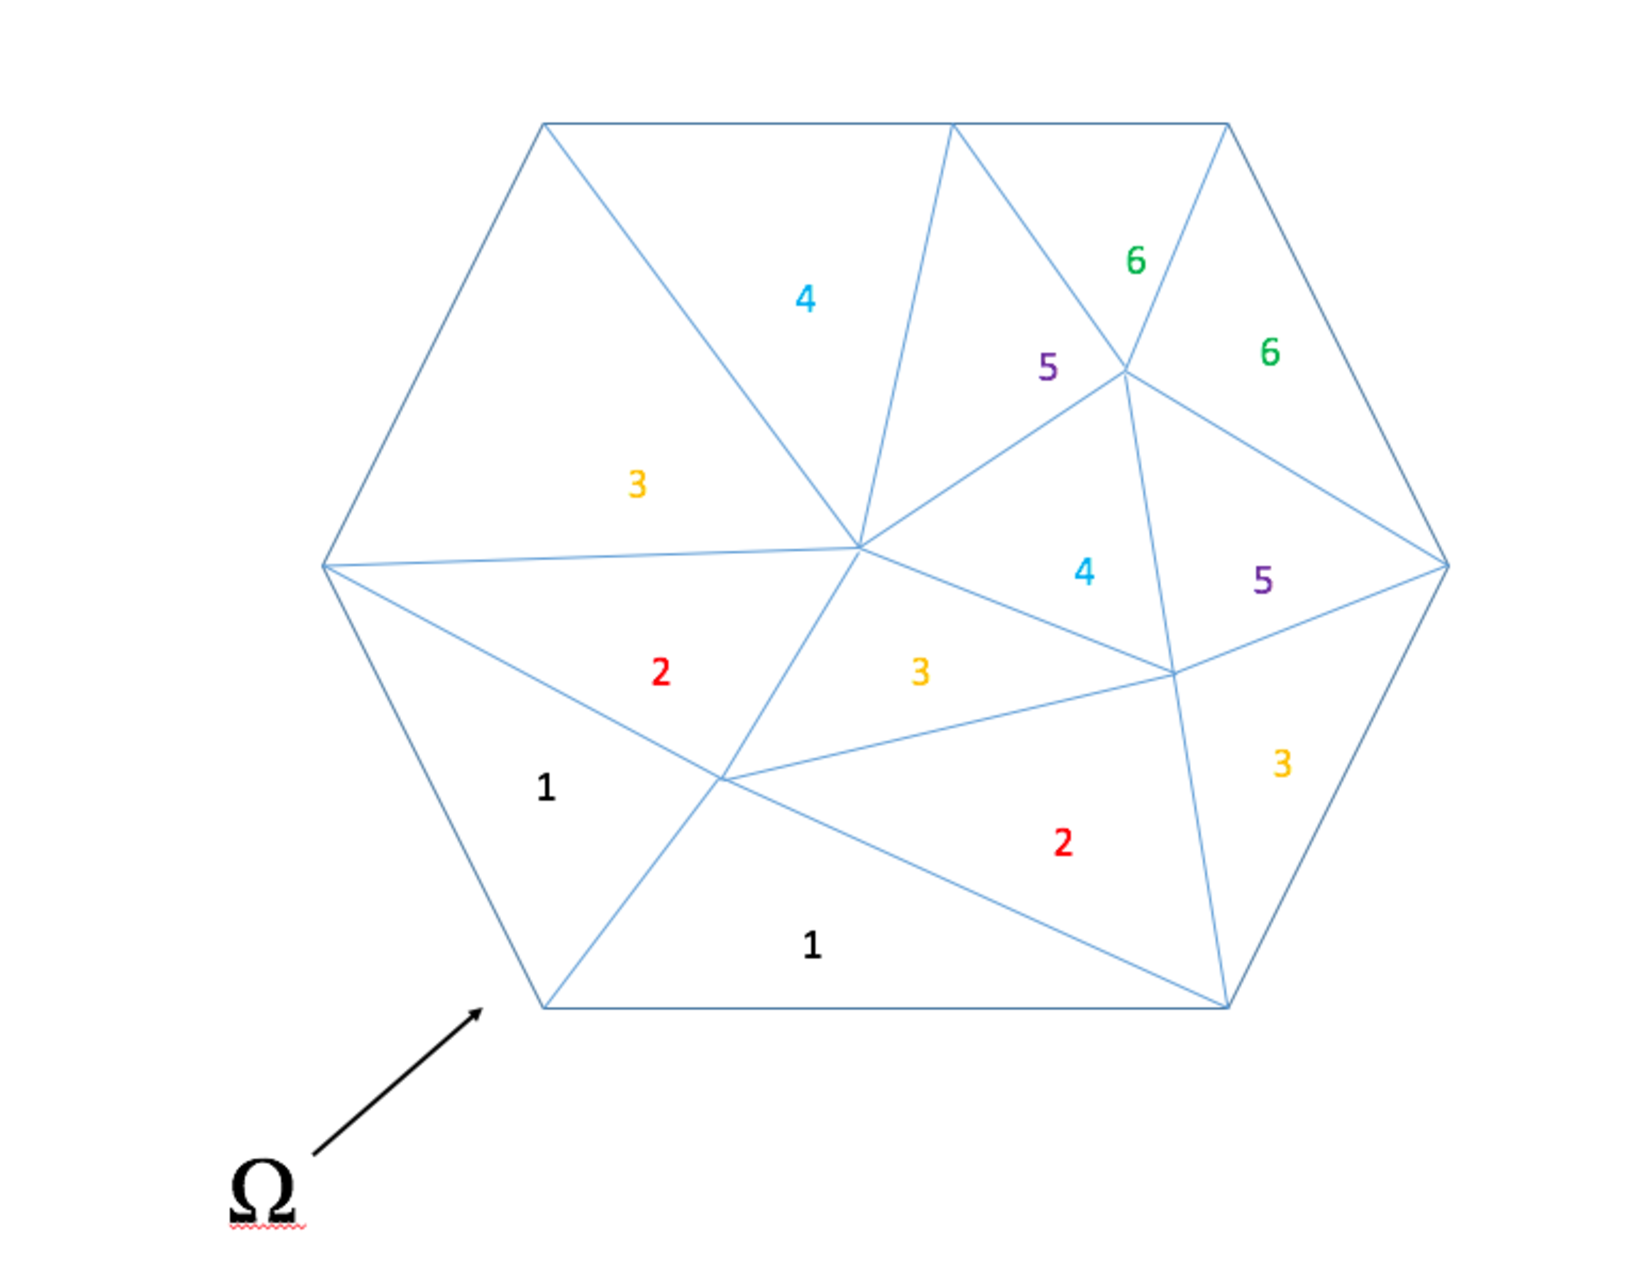
\includegraphics[scale = 0.27]{figures/UnstructureMesh.pdf}
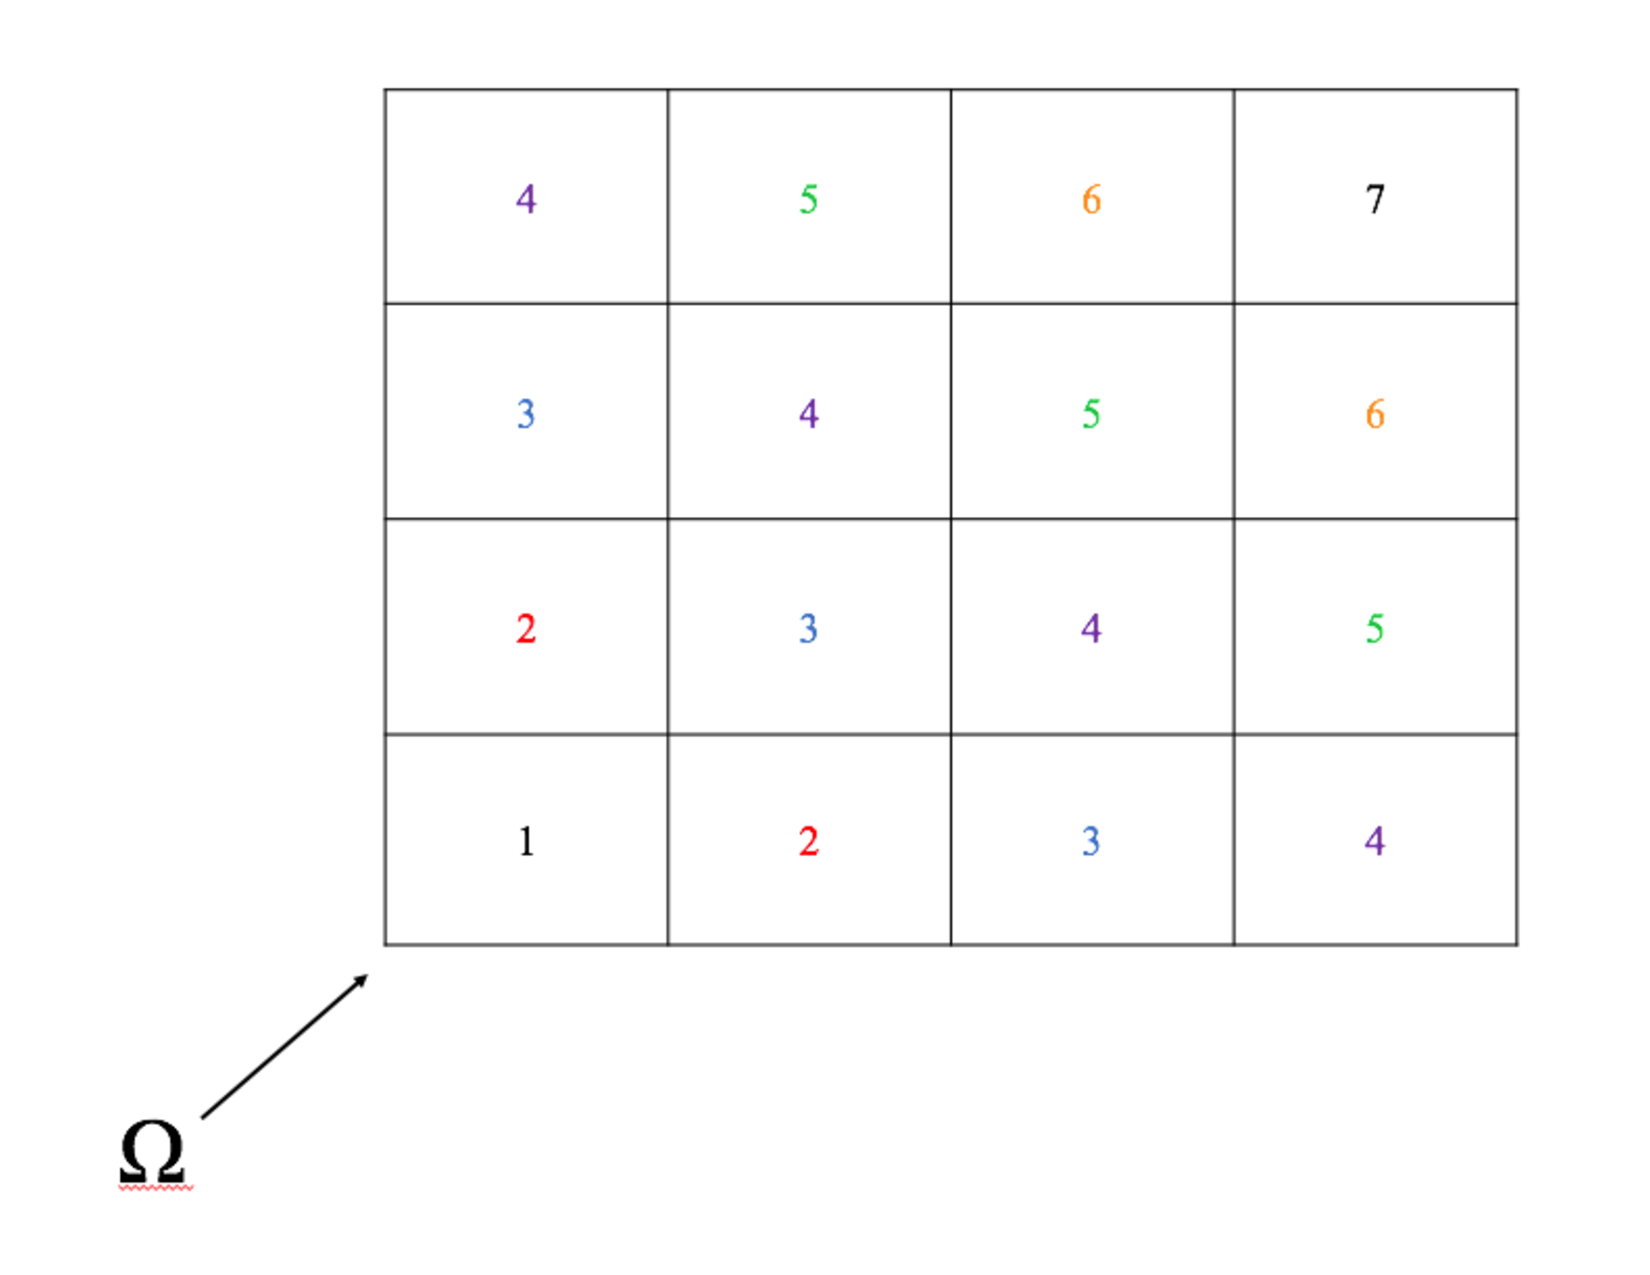
\includegraphics[scale = 0.27]{figures/StructuredMesh.pdf}
\caption{A demonstration of a sweep on a structured and unstructured mesh. }
\label{sweeps}
\end{figure}

The number in each cell represents the order in which the cells are solved. All cells must receive the solution downwind from them before solving for their own solution. This dependency can be represented and stored as a directed task dependence graph, shown in Fig.~\ref{tdg}.

\begin{figure}
\centering
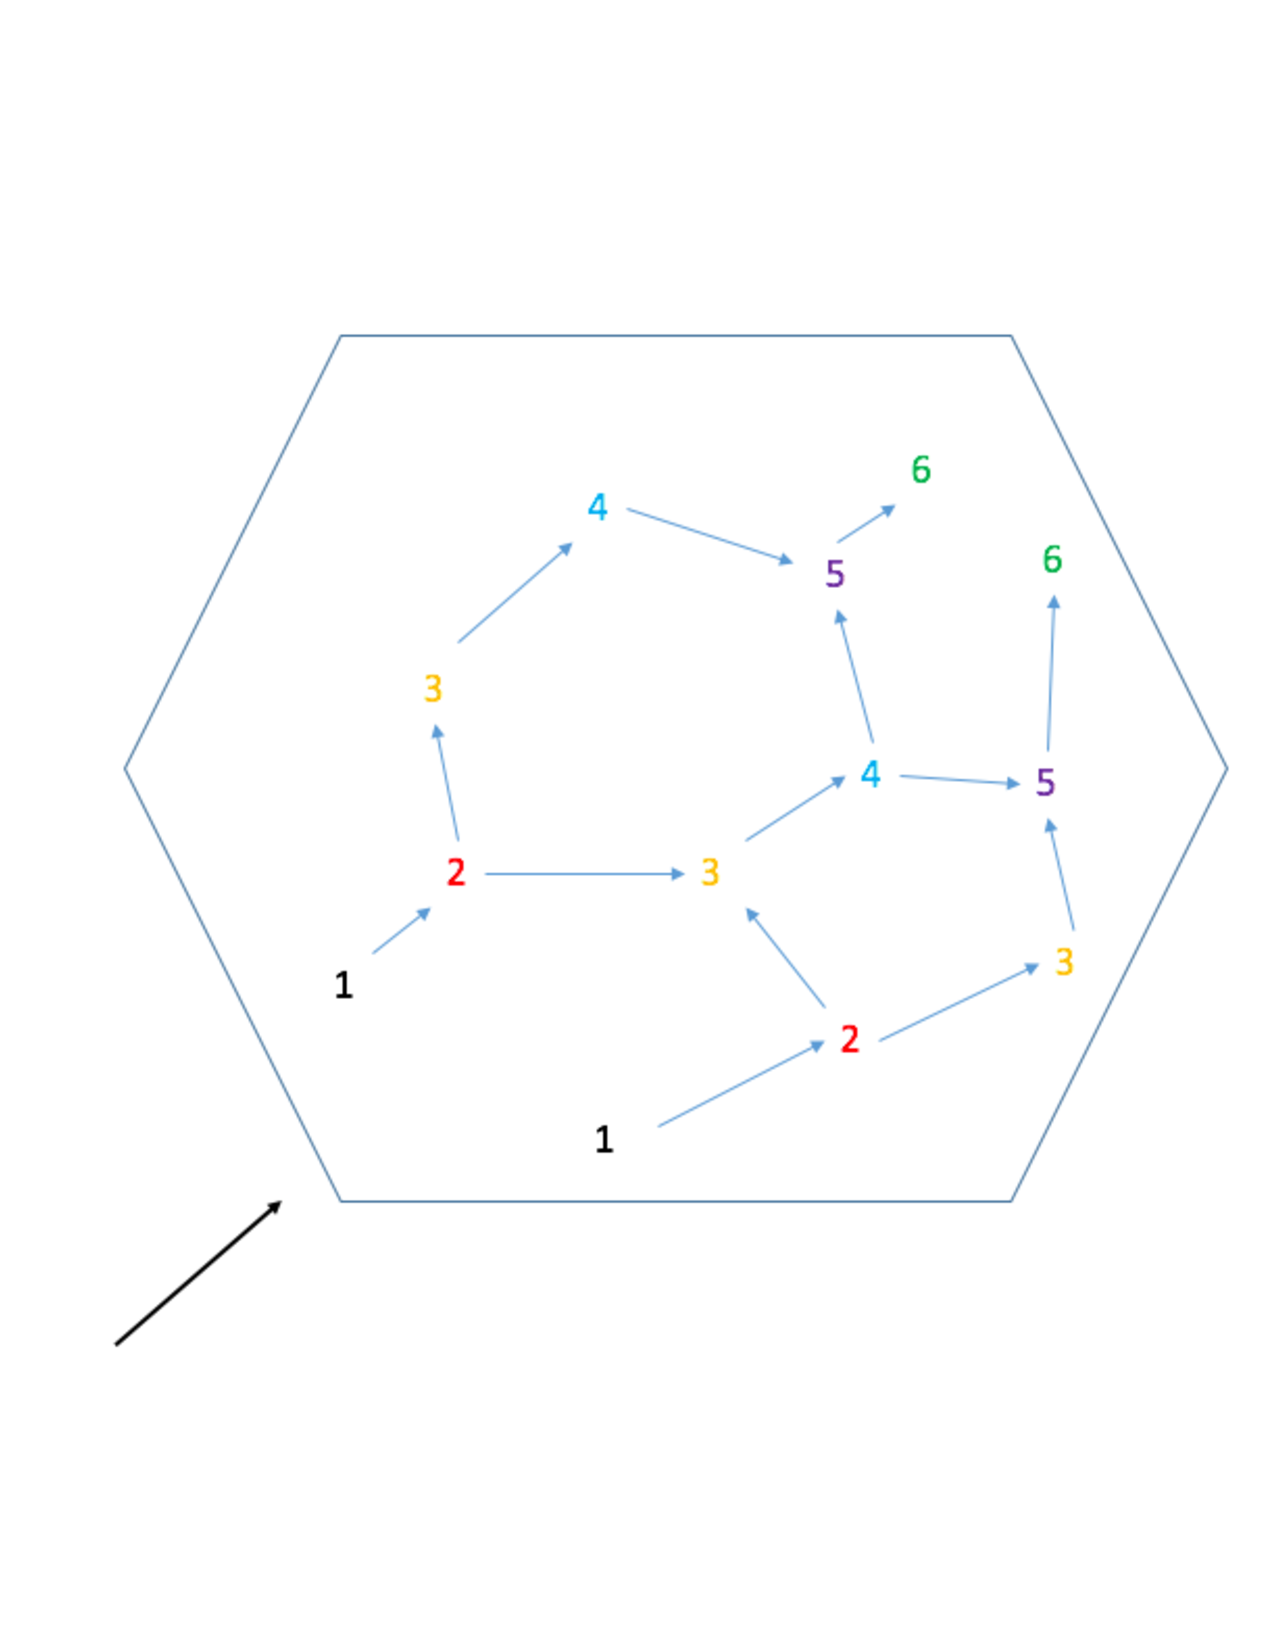
\includegraphics[scale = 0.4,trim = 0cm 3.5cm 0cm 3cm,clip]{figures/tdg.pdf}
\caption{A task dependence graph of the unstructured mesh example in Fig. \ref{sweeps}.}
\label{tdg}
\end{figure}

The order in which radiation in a cell is solved is given by a task dependence graph. Transport sweep can be performed on parallel architectures in order to obtain the solution faster, as well as distribute the memory to many processors for memory intensive cases. Provably-optimal transport sweeping has been described in \cite{mpadams2013} and demonstrated in PDT using logically-Cartesian meshes. Our work utilizes that transport sweep machinery but adapts it to unstructured meshes. Performing a transport sweep on an unstructured mesh presents two challenges: (1) performing a transport sweep on a massively parallel scale in an efficient manner and (2) keeping non-concave sub-domains due to leverage fromt he provably-optimal transport sweep algorithms. 

\subsection{The Parallel Transport Sweep}

A parallel sweep algorithm is defined by three properties \cite{mpadams2013} :
\begin{itemize}
\item partitioning: dividing the domain among available processors
\item aggregation: grouping cells, directions, and energy groups into tasks
\item scheduling: choosing which task to execute if more than one is available
\end{itemize}

The basic concepts of parallel transport sweeps, partitioning, aggregation, and scheduling, are most easily described in the context of a structured transport sweep. A structured transport sweep takes place on a Cartesian mesh. Furthermore, the work proposed utilizes aspects of the structured transport sweep.

If $M$ is the number of angular directions per octant, $G$ is the total number of energy groups, and $N$ is the total number of cells, then the total fine grain work units is $8MGN$. The factor of 8 is present as $M$ directions are swept for all 8 octants of the domain. The finest grain work unit is the calculation of a single direction and energy groups unknowns in a single cell, or $\psi_{m,g}$ for a single cell.

In a regular grid, we have the  number of cells in each Cartesian direction: $N_x, N_y, N_z$. These cells are aggregated into ``cellsets''. If $M$ is the total number of angular directions, $G$ is the total number of energy groups, and $N$ is the total number of cells, then the total fine grain work units is $8MGN$. The factor of 8 is present as $M$ directions are swept for all 8 octants of the domain. The finest grain work unit is the calculation of a single direction and energy groups unknowns in a single cell, or $\psi_{m,g}$ for a single cell.

Fine grain work units are aggregated into coarser-grained units called \textit{tasks}. A few terms are defined that describe how each variable is aggregated.
\begin{itemize}
\item $A_x = \frac{N_x}{P_x}$, where $N_x$ is the number of cells in $x$ and $P_x$ is the number of processors in $x$
\item $A_y = \frac{N_y}{P_y}$, where $N_y$ is the number of cells in $y$ and $P_y$ is the number of processors in $y$
\item $N_g = \frac{G}{A_g}$
\item $N_m = \frac{M}{A_m}$
\item $N_k = \frac{N_z}{P_z A_z}$
\item $N_k A_x A_y A_z = \frac{N_x N_y N_z}{P_x P_y P_z}$
\end{itemize}

It follows that each process owns $N_k$ cell-sets (each of which is $A_z$ planes of $A_x A_y$ cells), $8N_m$ direction-sets, and $N_g$ group-sets for a total of $8N_m N_g N_k$ tasks.

One task contains $A_x A_y A_z$ cells, $A_m$ directions, and $A_g$ groups. Equivalently, a task is the computation of one cellset, one groupset, and one angleset. One task takes a stage to complete.  This is particularly important when comparing sweeps to the performance models. 

Equation ~\eqref{paralleleff} approximately defines parallel sweep efficiency. This can be calculated for specific machinery and partitioning parameters by substituting in values calculated using Eqs.~\eqref{nfill},~\eqref{nidle}, and ~\eqref{ntasks}.
\begin{equation}\label{paralleleff}
\begin{split}
\epsilon &= \frac{T_{\text{task}} N_{\text{tasks}}}{[N_{\text{stages}}] [T_{\text{task}} + T_{\text{comm}}]} \\
            &=\frac{1}{[1+\frac{N_{\text{idle}}}{N_{\text{tasks}}}][1 + \frac{T_{\text{comm}}}{T_{\text{task}}}]}
\end{split}
\end{equation}

Equations ~\eqref{Tcomm} and \ref{Ttask} show how $T_{\text{comm}}$ and $T_{\text{task}}$ are calculated:
\begin{equation}
T_{\text{comm}} = M_L T_{\text{latency}} + T_{\text{byte}} N_{\text{bytes}}
\label{Tcomm}
\end{equation}
\begin{equation}
T_{\text{task}} = A_x A_y A_z A_m A_g T_{\text{grind}}
\label{Ttask}
\end{equation}
where $T_{\text{latency}}$ is the message latency time, $T_{\text{byte}}$ is the time required to send one byte of message, $N_{\text{bytes}}$ is the total number of bytes of information that a processor must communicate to its downstream neighbors at each stage, and $T_{\text{grind}}$ is the time it takes to compute a single cell, direction, and energy group. $M_L$ is a latency parameter that is used to explore performance as a function of increased or decreased latency. If a high value of $M_L$ is necessary for the performance model to match computational results, improvements should be made in code implementation.

\subsubsection{KBA Partitioning for Structured Grids}

Several parallel transport sweep codes use KBA partitioning in their sweeping, such as Denovo \cite{denovo} and PARTISN \cite{partisn}. The KBA partitioning scheme and algorithm was developed by Koch, Baker, and Alcouffe \cite{partisn}.

The KBA algorithm traditionally chooses $P_z = 1, A_m = 1, G = A_g = 1, A_x = N_x/P_x, A_y = N_y/P_y$, with $A_z$ being the selectable number of z-planes to be aggregated into each task. With $N_k = N_z/A_z$, each processor performs $N_{\text{tasks}} = 8MN_k$ tasks. With the KBA algorithm, $2MN_k$ tasks are pipelined from a given corner of the 2D processor layout. The far corner processor remains idle for the first $P_x + P_y - 2 $ stages, which means that an octant-pair (or quadrant) sweep completes in $2MN_k + P_x + P_y - 2$ stages. If an octant-pair sweep does not begin until the previous pair's finishes, the full sweep requires $8MN_k + 4(P_x+P_y-2)$ stages, which means the KBA parallel efficiency is:
\begin{equation}
\varepsilon_{KBA} = \frac{1}{[1+\frac{4(P_x+P_y-2)}{8MN_k}][1+\frac{T_{\text{comm}}}{T_{\text{task}}}]}
\label{eKBA}
\end{equation}

%%%%%%%%%%%%%%%%%%%%%%%%%%%%%%%%%%%%%%%%%%%%%%%%%%%%%%%%%%%%%%%%%%%%%
\subsubsection{The Structured Transport Sweep in PDT}
%%%%%%%%%%%%%%%%%%%%%%%%%%%%%%%%%%%%%%%%%%%%%%%%%%%%%%%%%%%%%%%%%%%%%
The minimum possible number of stages for given partitioning parameters $P_i$ and $A_j$ is $2 N_{\text{fill}}+N_{\text{tasks}}$. $N_{\text{fill}}$ is both the minimum number of stages before a sweepfront can reach the center-most processors and the number needed to finish a direction's sweep after the center-most processors have finished. Equations~\eqref{nfill}, ~\eqref{nidle}, and~\eqref{ntasks} define $N_{\text{fill}}$, $N_{\text{idle}}$, and $N_{\text{tasks}}$:
\begin{equation}
N_{\text{fill}} = \frac{P_x + \delta_x}{2} - 1 + \frac{P_y + \delta_y}{2} - 1 + N_k (\frac{P_z + \delta_z}{2} - 1)
\label{nfill}
\end{equation}
\begin{equation}
N_{\text{idle}} = 2 N_{\text{fill}}
\label{nidle}
\end{equation}
\begin{equation}
N_{\text{tasks}} = 8 N_m N_g N_k
\label{ntasks}
\end{equation}
where $\delta_u$ is 1 for $P_u$ odd, and 0 for $P_u$ even.

When using KBA, $P_z$ is fixed to 1, and with hybrid KBA, $P_z$ is fixed to 2. Volumetric partitioning means that $P_z$ is greater than two. Figure \ref{partitioning} shows three different partitioning schemes used in transport sweeps, KBA (which is defined in the previous section), volumetric non-overloaded, and volumetric overloaded. Volumetric non-overloaded requires that all cells owned by a processor are contiguous, where as volumetric non-overloaded partitioning does not have this restriction.  

\begin{figure}
\centering
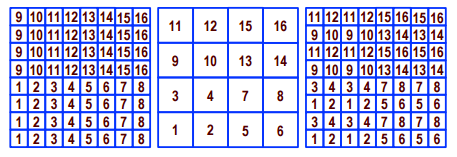
\includegraphics[scale = 0.75]{figures/Partitioning.png}
\caption{Three different partitioning schemes in 2D, from left to right: KBA, volumetric non-overloaded, and volumetric overloaded \cite{mpadams2015}.}
\label{partitioning}
\end{figure}

For a thorough and complete description of partitioning, aggregation, and scheduling in PDT, please refer to \cite{mpadams2015}.
%The overloaded volumetric partitioning proceeds as follows:
%
%\begin{enumerate}
%\item In a 2D (3D) domain, cellsets are divided into 4 (8) spatial quadrants (octants), with an equal number of cellsets in each  SQO (SQO is defined as a spatial quadrant or octant).
%\item Assign 1/4 of the processors (1/8) in 3D to each SQO. 
%\item Choose the individual overload factors $\omega_x, \omega_y, \text{and } \omega_z$ and individual processor counts $P_x, P_y, \text{and }P_z$, such that $\omega_x \omega_y \omega_z = \omega_r$ and $P_x P_y P_z = P$, with all $P_u$ even. $\omega_u$ is defined as the number of cellsets assigned to each $P_u$.
%\item An array of $\omega_x\cdot\omega_y\cdot\omega_z$ ``tiles'' in each SQO. Each tile is an array of $1/2 P_x \cdot 1/2 P_y \cdot 1/2 P_z$ cellsets. These cellsets are mapped one-to-one to the $1/2 P_x \cdot 1/2 P_y \cdot 1/2 P_z$ processors assigned to the SQO, using the same mapping in each tile.
%\end{enumerate}
%Each tile has a logically identical layout of cellsets, and each processor owns exactly one cellset in each tile in its SQO. This makes each processor responsible for $\omega_r$ cellsets.
%
%In order to properly outline the optimal scheduling rules, the variables $X,Y, \text{and } Z$ are defined as $P_u/2$ for each respective direction $u = x,y,z$. This splits up the processor layout into octants, where each processor has an index $(i,j,k)$ determining where it is in the layout. Tiles are also indexed and referred to in the same way with the notation $T(i,j,k)$. 
%
%The optimal scheduling algorithm rules are as follows:
%\begin{enumerate}
%\item If $i \leq X$, then tasks with $\Omega_x > 0$ have priority, while for $i > X$, tasks with $\Omega_x < 0$ have priority.
%\item If multiple ready tasks have the same sign on $\Omega_x$, apply rule 1 to $j,Y,\Omega_y$.
%\item If multiple ready tasks have the same sign on $\Omega_x$ and $\Omega_y$, apply rule 1 to $k,Z, \Omega_z$. 
%\item If multiple tasks are ready in the same octant, then priority goes to the cellset for which the priority octant has greatest downstream depth.
%\item If multiple ready tasks are in the same octant and have the same downstream depth of graph in $x$, then priority goes to the cellset for which the priority octant has greatest downstream depth of graph in $y$.
%\item If multiple ready tasks are in the same octant and have the same downstream depth of graph in $x$ and $y$, then priority goes to the cellset for which priority octant has greatest depth of graph in $z$.
%\end{enumerate}
%This ensures that each SQO orders the octants: the one it can start right away ($A$), three that have one sign difference from $A (B,C,$ and $D)$, three that have two sign differences ($\bar D, \bar C, \bar B$), and one in opposition to its primary ($\bar A$). For example, if octant $A$ is octant $(+x, +y, +z)$, then it's secondary octants (only one sign change at a time) would be octants $(-x, +y, +z)$, $(+x,-y,+z)$ and $(+x,+y,-z)$.
%
%There are three constraints in order to achieve the optimal stage count. In these constraints, $M = \omega_g \omega_m/8$, which is the number of tasks per octant per cellset.
%\begin{enumerate}
%\item $ M \geq 2(Z-1)$
%\item $\omega_z M \geq 2(Y-1)$
%\item If $\omega_x > 1$, then $\omega_y \omega_z M \geq X$
%\end{enumerate}
%Constraint 1 ensures that there is no idle time between a processor finishing an octant's work in one tile and beginning that octant's work on the next tile in the same tile-column; processor $P(1,Y,1)$ finishing its tile $T(1,\omega_y,1)$ octant $C$ work and beginning its octant $B$ work; processor $P(X,1,1)$ finishing its tile $T(\omega_x,1,1)$ octant $D$ work and beginning its octant $B$ work. Constraint 2 ensures that there is no idle time time between a processor finishing an octant's work for one $z$ column of tiles and beginning that octant's work on the next column; processor $P(X,1,1)$ finishing its tile $T(\omega_x,1,1)$ octant D work available to it and beginning its octant $C$ work. Constraint 3 ensures that there is no idle time between a processor finishing an octant's work for one $yz$ plane of tiles and beginning that octant's work in the next plane.
%
%As a result of these constraints, there is no idle time for a variety of situtations. At large processor counts, the product $\omega_m \omega_g$ must be large, which requires $N_m N_g$ be large. This means that a weak scaling series refined only in space, but only coarsely refined in angle and energy, will eventually fail the constraints.
%
%The optimal efficiency formula changes slightly from the KBA and hybrid KBA partitioning method in order to account for the overload factors. The only change is in the $\frac{N_{idle}}{N_{tasks}}$ term, as shown in Eq. ~\eqref{overloadpartitioning}. 
%\begin{equation}
%\varepsilon_{opt} = \frac{1}{[1+\frac{P_x+P_y+P_z-6}{\omega_g \omega_m \omega_r}][1+\frac{T_{\text{comm}}}{T_{\text{task}}}]}
%\label{overloadpartitioning}
%\end{equation}


%%%%%%%%%%%%%%%%%%%%%%%%%%%%%%%%%%%%%%%%%%
\subsubsection{The Unstructured Transport Sweep}
%%%%%%%%%%%%%%%%%%%%%%%%%%%%%%%%%%%%%%%%%%
In an unstructured mesh, the number of cells cannot be described in the same way as a structured mesh. In PDT, the 2D
geometry is first subdivided into subsets, which are just rectangular subdomains. Within each subset, an unstructured mesh is generated (using Triangle) and then extruded in 3D. These subsets become the $N_x, N_y, N_z$ equivalent for an structured mesh. The spatial aggregation in a PDT unstructured mesh is done by aggregating subsets into cellsets. 

While the PDT transport sweep on structured grids has scaled well out to 768,000 cores, similar levels of parallel scaling have not been achieved using unstructured sweeps yet. Further work is being done to determine how well PDT scales on unstructured meshes. The load balancing algorithm described in this paper was the first step to scaling on unstructured meshes.

%%%%%%%%%%%%%%%%%%%%%%%%%%%%%%
\section{Load Balancing Method}
The capability for PDT to generate and run on an unstructured mesh is important because it allows us to run problems without having to conform our mesh to the problem as much. The idea is to have a logically Cartesian grid (creating orthogonal ``subsets'') with an unstructured mesh inside each subset. These logically Cartesian subdomains are obtained using cut planes in 3D and cut lines in 2D. Figure \ref{grid} demonstrates this functionality. It is decomposed into 3 subsets in x and 3 in y, with the first two subsets meshed using the Triangle Mesh Generator\cite{triangle}, a 2D mesh generator.

\begin{figure}
\centering
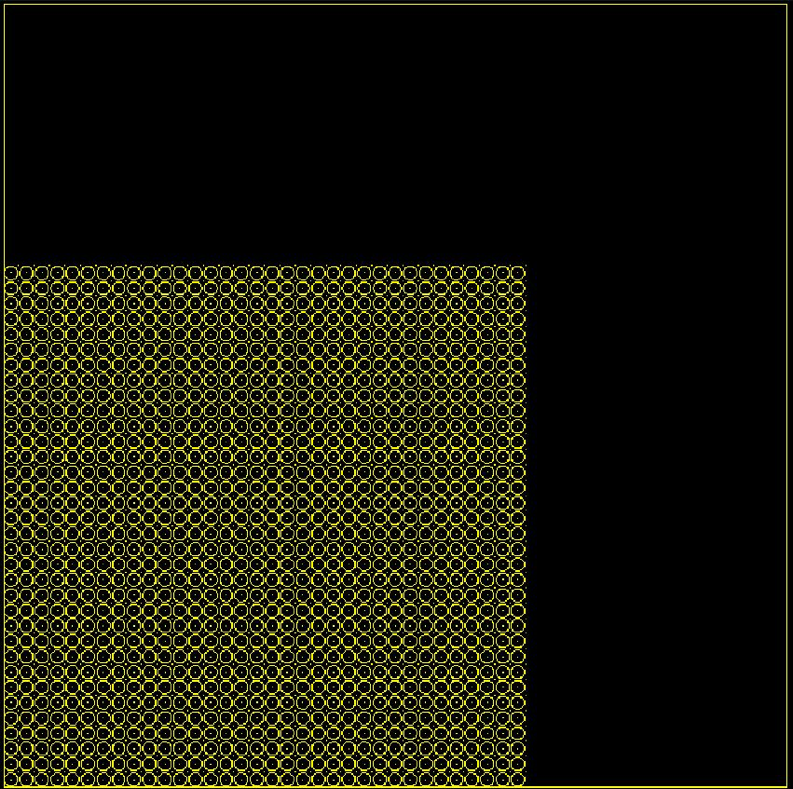
\includegraphics[scale = 0.5]{figures/lattice.png}
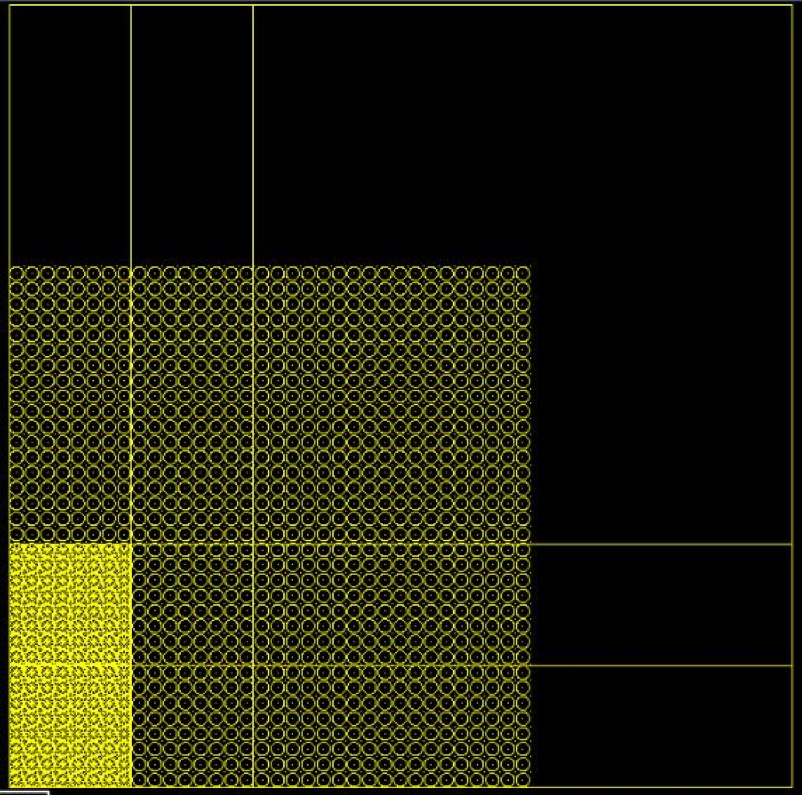
\includegraphics[scale = 0.5]{figures/subsetlattice.png}
\caption{A PSLG describing a fuel lattice, and with an orthogonal ``subset" grid imposed on the PSLG.}
\label{grid}
\end{figure}

This orthogonal grid is superimposed and each subset is meshed in parallel.  Subsets are now the base structured unit when calculating our parallel efficiency. Discontinuities along the boundary are fixed by ``stitching'' hanging nodes, creating degenerate polygons along subset boundaries. Because PDT's spatial discretization employs Piece-Wise Linear Discontinuous (PWLD) finite element basis functions, there is no problem solving on degenerate polygons. 

When using the unstructured meshing capability in PDT, the input geometry is described by a Planar Straight Line Graph (PSLG)\cite{triangle}. After superimposing the orthogonal grid, a PSLG is created for each subset, and meshed. Because the input's and each subset's PSLG must be described and meshed in 2D, the mesh can be extruded in the $z$ dimension in order to give us the capability to run on 3D problems. Obviously, this is not as good as general an unstructured grid as a tetrahedral grid, but for many problems (e.g., reactor problems), it is a useful capability to have and it can be employed to assess load-balancing algorithm. 

When discussing the parallel scaling of transport sweeps, a load balanced problem is of great importance. A load balanced problem has an equal number of degrees of freedom per processor. Load balancing is important in order to minimize idle time for all processes by equally distributing (as much as possible) the work on each process.  For the purposes of unstructured meshes in PDT, we are looking to ``balance'' the number of cells. Ideally, each process will be responsible for an equal number of cells. 

If the number of cells in each subset can be reasonably balanced, then the problem is effectively load balanced. The Load Balance algorithm described below details how the subsets will be load balanced. In summary, the procedure of the algorithm involves moving the initially user specified $x$ and $y$ cut planes, re-meshing, and iterating until a reasonably load balanced problem is obtained.  Equation \ref{metric_def} shows the equation for calculating the load balancing metric, which dictates how balanced or unbalanced the problem is.
\begin{equation}
f =\frac{\underset{ij}{\text{max}}(N_{ij})}{\frac{N_{tot}}{I\cdot J}},
\label{metric_def}
\end{equation}
where $f$ is the load balance metric, $N_{ij}$ is the number of cells in subset $i,j$, $N_{tot}$ is the global number of cells in the problem, and $I$ and $J$ are the total number of in the $x$ and $y$ direction, respectively. The metric is a measure of the maximum number of cells per subset divided by the average number of cells per subset.

The load balancing algorithm moves cut planes based on two sub-metrics, $f_I$ and $f_J$. Equation ~\eqref{submetric} defines these two parameters:
\begin{align}
f_I &= \underset{i}{\text{max}}[\sum_{j} N_{ij}]/\frac{N_{tot}}{I} \notag \\
f_J &= \underset{j}{\text{max}}[\sum_{i} N_{ij}]/\frac{N_{tot}}{J}.
\label{submetric}
\end{align}

$f_I$ is calculated by taking the maximum number of cells per column and dividing it by the average number of cells per column. $f_j$ is calculated by taking the maximum number of cells per row and dividing it by the average number of cells per row. If these two numbers are greater than predefined tolerances, the cut lines in the respective directions are redistributed. Once redistribution and remeshing occur, a new metric is calculated. This iterative process occurs until a maximum number of iterations is reached, or until $f$ converges within the user defined tolerance. The Load Balance algorithm behaves as follows:

\lstinputlisting[language = C++, basicstyle = \footnotesize]{loadbalance.cc}

\noindent\begin{minipage}{\textwidth}
\textbf{Redistribute:} A function that moves cut lines in either X or Y. \\
\begin{algorithmic}
\STATE \textbf{Input:}CutLines (X or Y vector that stores cut lines). 
\STATE \textbf{Input:} num\_tri\_row or num\_tri\_col, \# of tri in each row/col
\STATE \textbf{Input:} The total number of triangles in the domain, $N_{tot}$
\STATE stapl::array\_view num\_tri\_view, over num\_tri\_row/column
\STATE stapl::array\_vew offset\_view
\STATE stapl::partial\_sum(num\_tri\_view) \COMMENT {Perform prefix sum}\\
\COMMENT {We now have a cumulative distribution stored in offset\_view}
\FOR {$i = 1$ :CutLines.size()-1}

	\STATE vector $<$double$>$ pt1 = [CutLines(i-1), offset\_view(i-1)]
	\STATE vector $<$double$>$ pt2 = [CutLines(i), offset\_view(i)]
	\STATE ideal\_value = $i\cdot \frac{N_{tot}}{\text{CutLines.size()}-1}$\\
         \COMMENT{Calculate X-intersect of the line formed by pt1 and pt2}\\
          \COMMENT{and the line y = ideal\_value.}
	\STATE X-intersect(pt1,pt2,ideal\_value)	\STATE CutLines(i) = X-intersect
\ENDFOR
\end{algorithmic}
\end{minipage} 


%%%%%%%%%%%%%%%%%%%%%%%%%%%%%%%%%%%%%%%%%%%%%%%%%%%%%%%%%%%%%%%%%%%%%%%%%%%%%%%%
\section{Results and Analysis}

The following sections will showcase the metric behavior and convergence for three test cases, solution verification for pure absorber and pure scatterer 2D slab problems, and the new unstructured meshing capability both in 2D and 3D.

\subsection{Description of Test Cases}
\label{sec:convergence}
In order to showcase the behavior of the load balancing metric, calculated by Eq. \ref{metric_def} three test cases are presented. Figure \ref{opp} shows the first test case, a 20 cm by 20 cm domain with two pins in opposite corners of the domain. Figure \ref{same} shows the same size domain but with the pins on the same side.These are two theoretically very unbalanced cases, as geometrically there are two features located distantly from each other with an empty geometry throughout the rest of the domain. Figure \ref{lattice} shows a lattice and reflector, which due to it's denser and repeated geometry, theoretically is a more balanced problem. 

A series of 162 inputs was constructed for each case. These inputs are constructed by varying the maximum triangle area from the coarsest possible (refers to Triangle utilizing the fewest possible triangles to mesh the geometry) to 0.01 cm\textsuperscript{2} and the number of subsets, $N$ from 2$\times$2 to 10$\times$10.
\begin{figure}
\centering
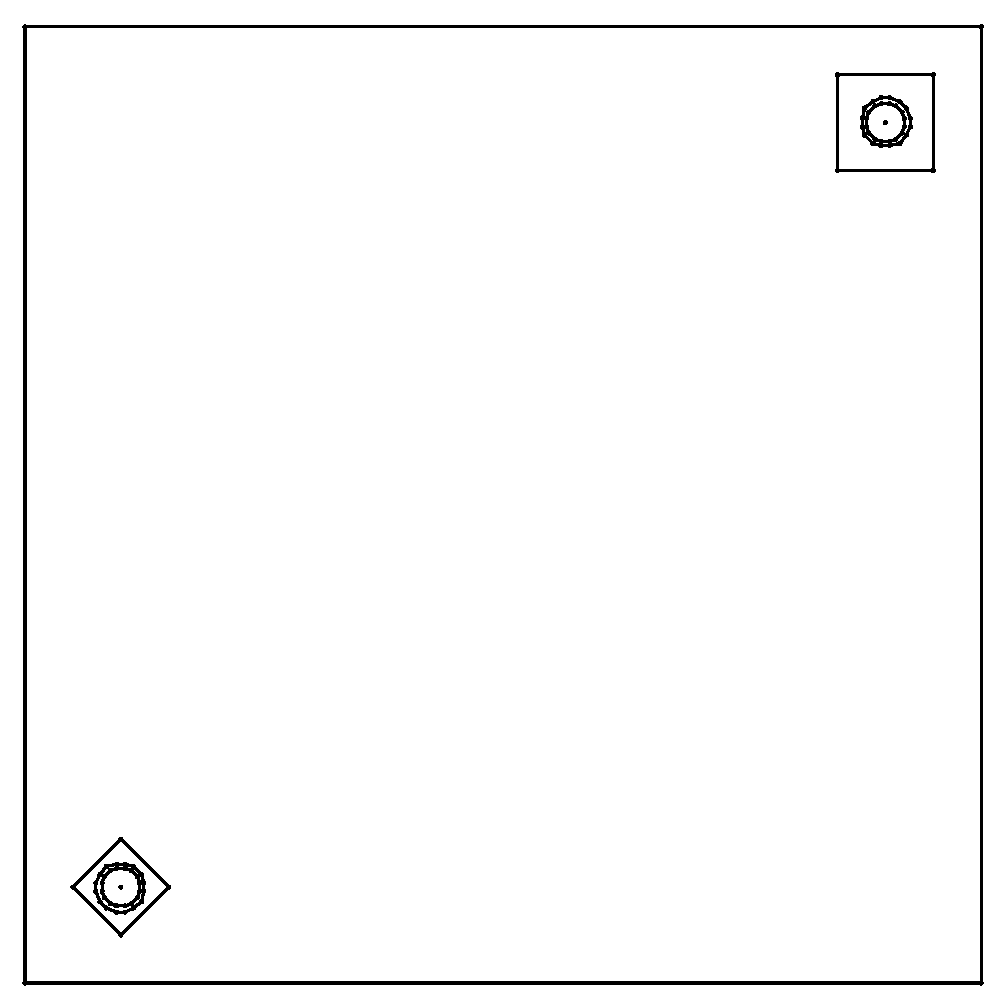
\includegraphics[scale = 0.5]{figures/unbalanced_lattice.eps}
\caption{The first test case used in order to test effectiveness and convergence of the load balancing metric.}
\label{opp}
\end{figure}

\begin{figure}
\centering
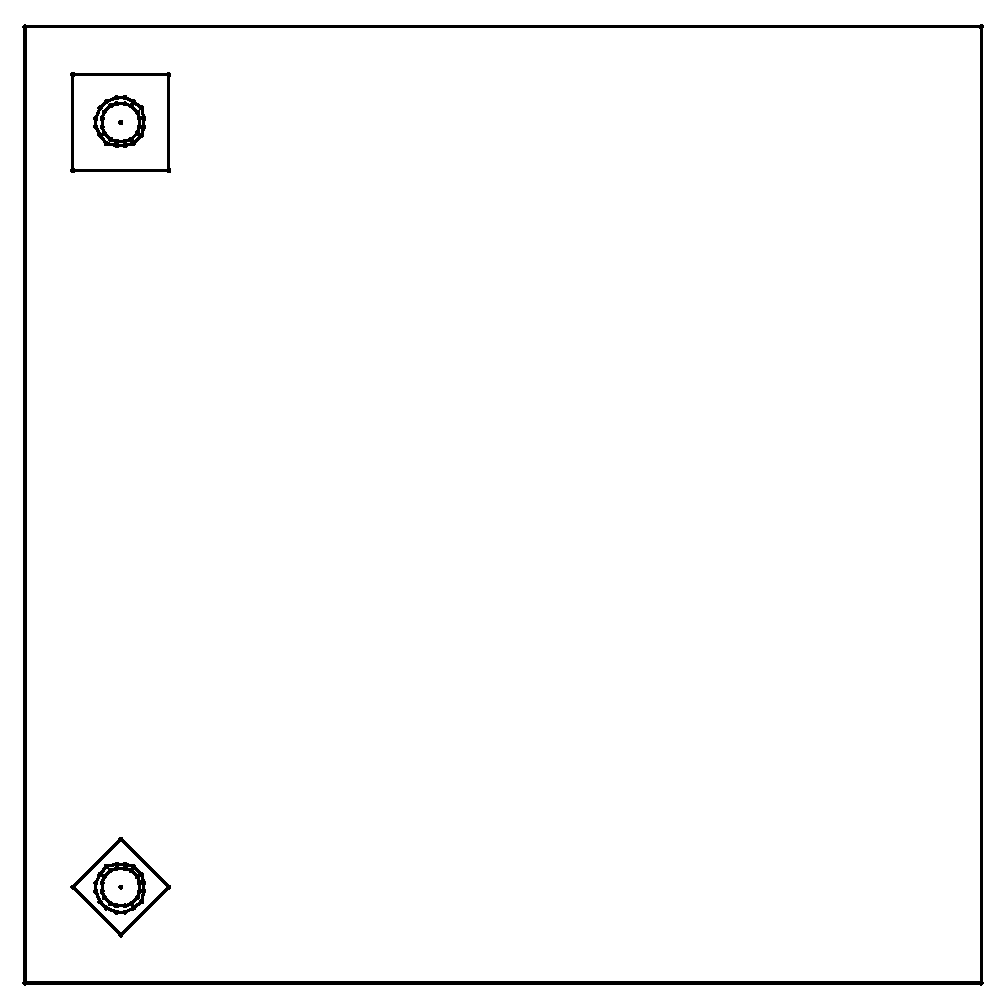
\includegraphics[scale = 0.5]{figures/unbalanced_pins_same_side.eps}
\caption{The second test case used in order to test effectiveness and convergence of the load balancing metric.}
\label{same}
\end{figure}


\begin{figure}
\centering
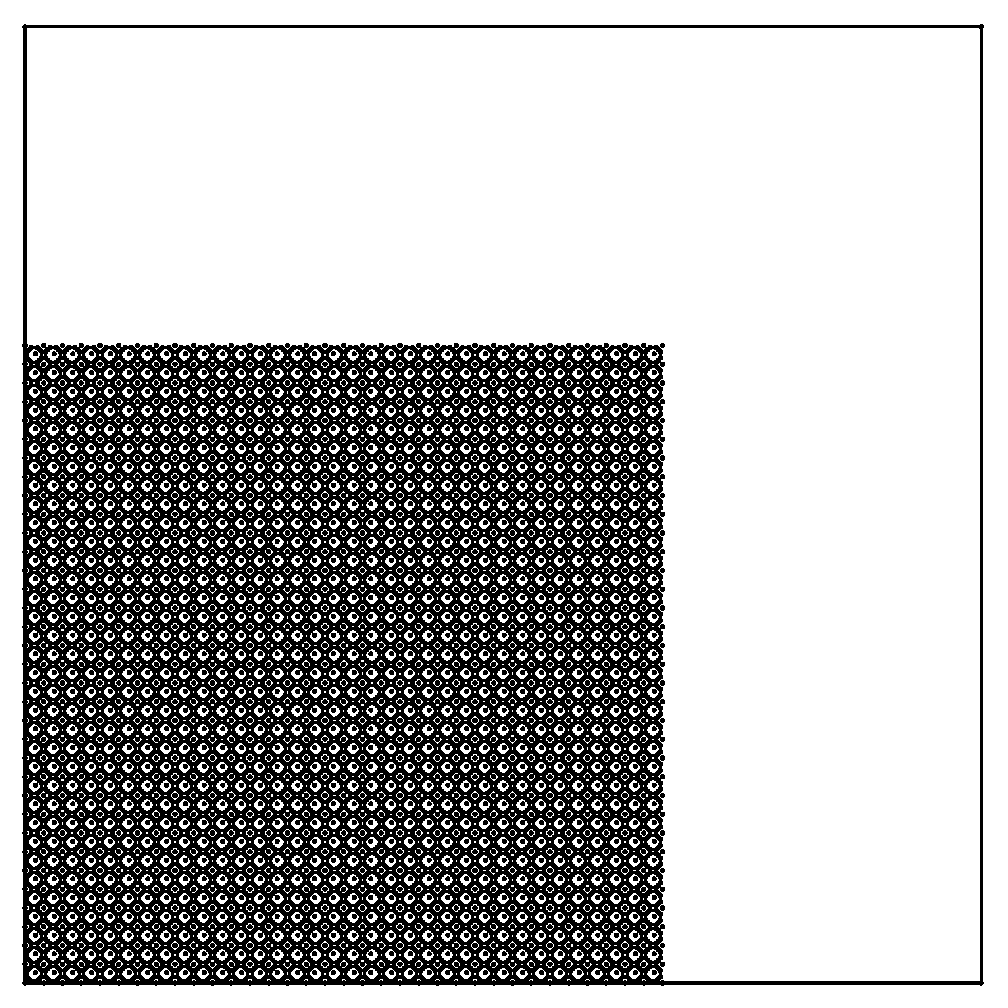
\includegraphics[scale = 0.5]{figures/lattice-12-shifted.eps}
\caption{The third test case used in order to test effectiveness and convergence of the load balancing metric.}
\label{lattice}
\end{figure}

\subsection{Load Balancing Analysis}

For each test case, the 162 input inputs are run twice, once with no load balancing iterations, and once with ten load balancing iterations. The best metric is reported and recorded. Three figures for each test cases are presented below: the first figure will show the metric behavior for no iterations, the second figure will show the metric behavior for each input run with ten load balancing iterations, and the third figure will show a ratio of the ten iteration runs over the no iteration runs.

Figure \ref{oppnoiter} shows the metric behavior for Fig. \ref{opp}. The maximum metric value is 24.7650, and occurs when Fig. \ref{opp} is run with 8x8 subsets and a maximum triangle area of 1.6 cm\textsuperscript{2}. The minimum metric value is 1.0016 and occurs when Fig. \ref{opp} is run with 4x4 subsets and a maximum triangle area of 0.04 cm\textsuperscript{2}. The z axis in all figures is the value of the metric.

\begin{figure}
\centering
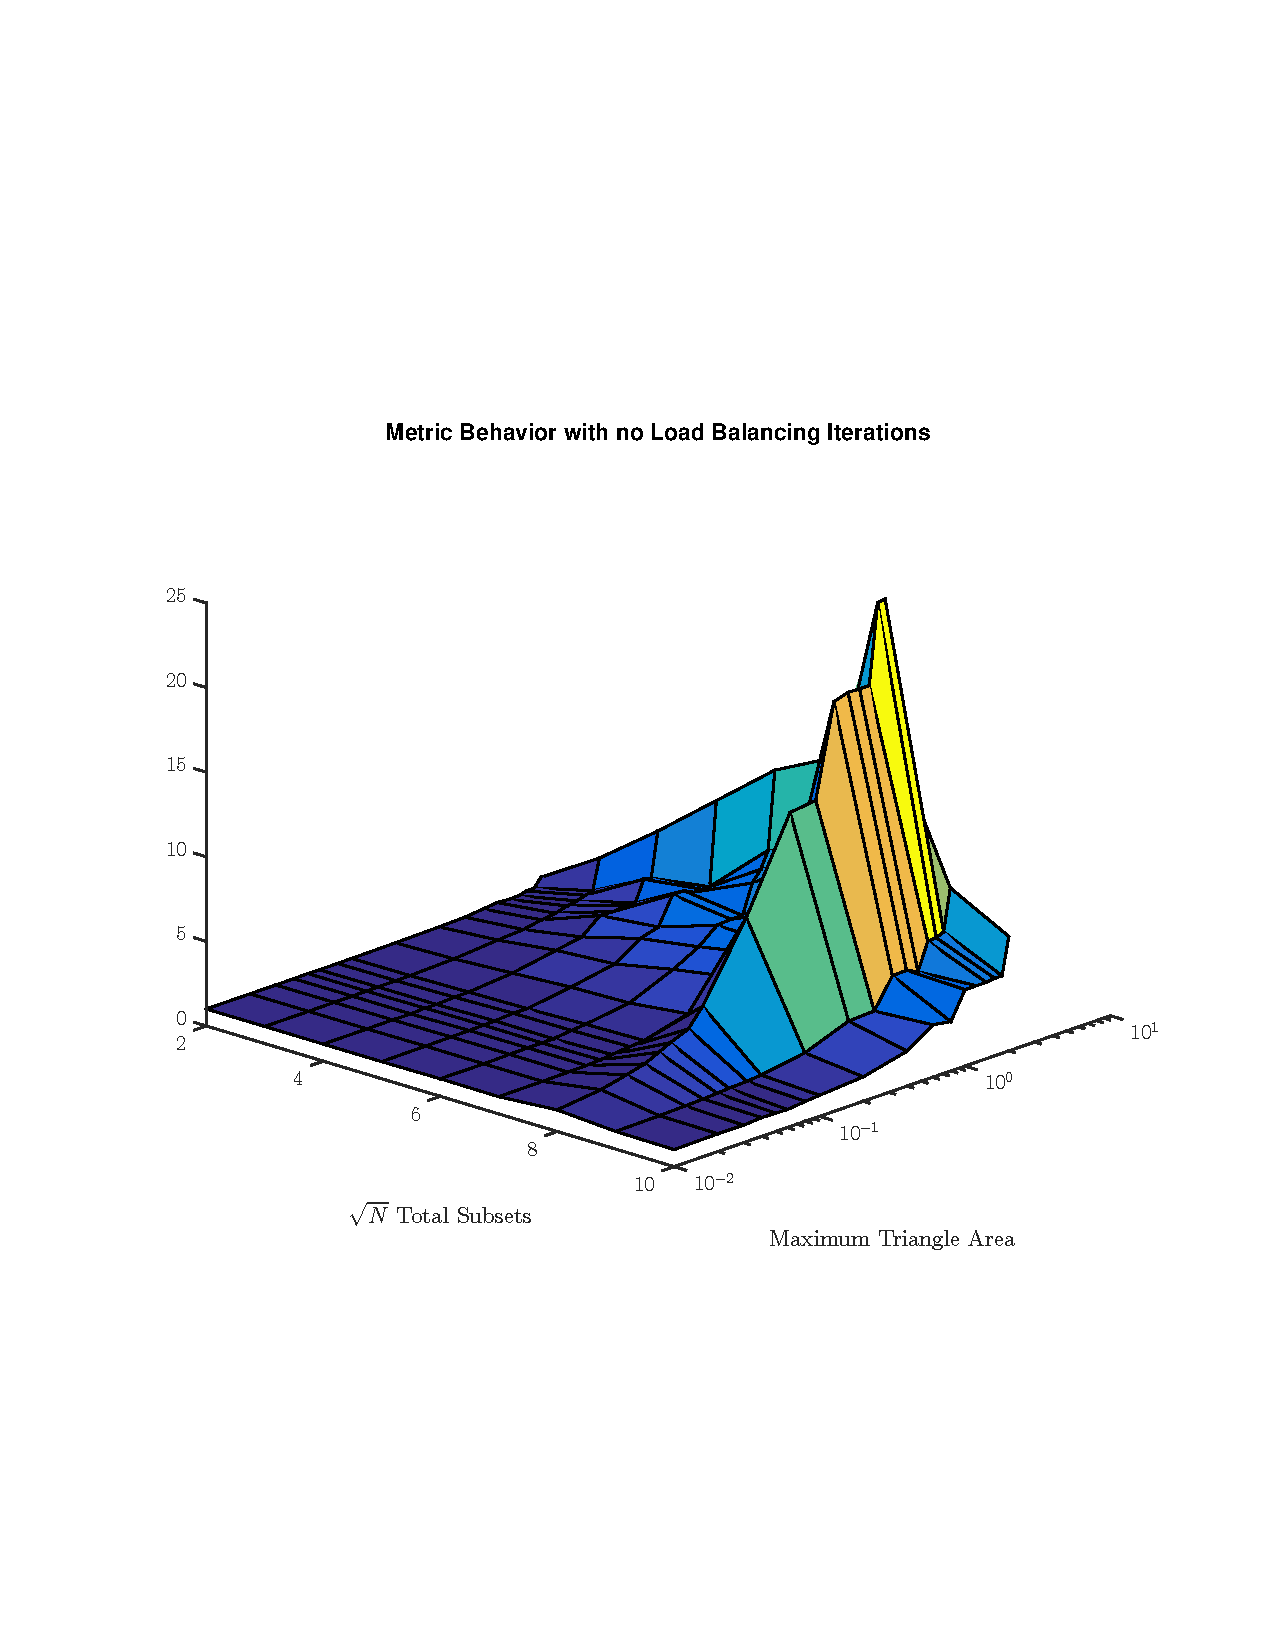
\includegraphics[width=85mm, trim = 0cm 5cm 0cm 5cm,clip]{figures/OppNoIter.pdf}
\caption{The metric behavior of the first test case run with no load balancing iterations.}
\label{oppnoiter}
\end{figure}

Figure \ref{oppiter} shows the metric behavior for Fig. \ref{opp} after 10 load balancing iterations. The maximum metric value is 5.0538 and occurs when Fig. \ref{opp} is run with 10x10 subsets and a maximum triangle area of 1.2 cm\textsuperscript{2}. The minimum metric value is 1.0017 and occurs when Fig. \ref{opp} is run with 4x4 subsets and a maximum triangle area of 0.04 cm\textsuperscript{2}.

\begin{figure}
\centering
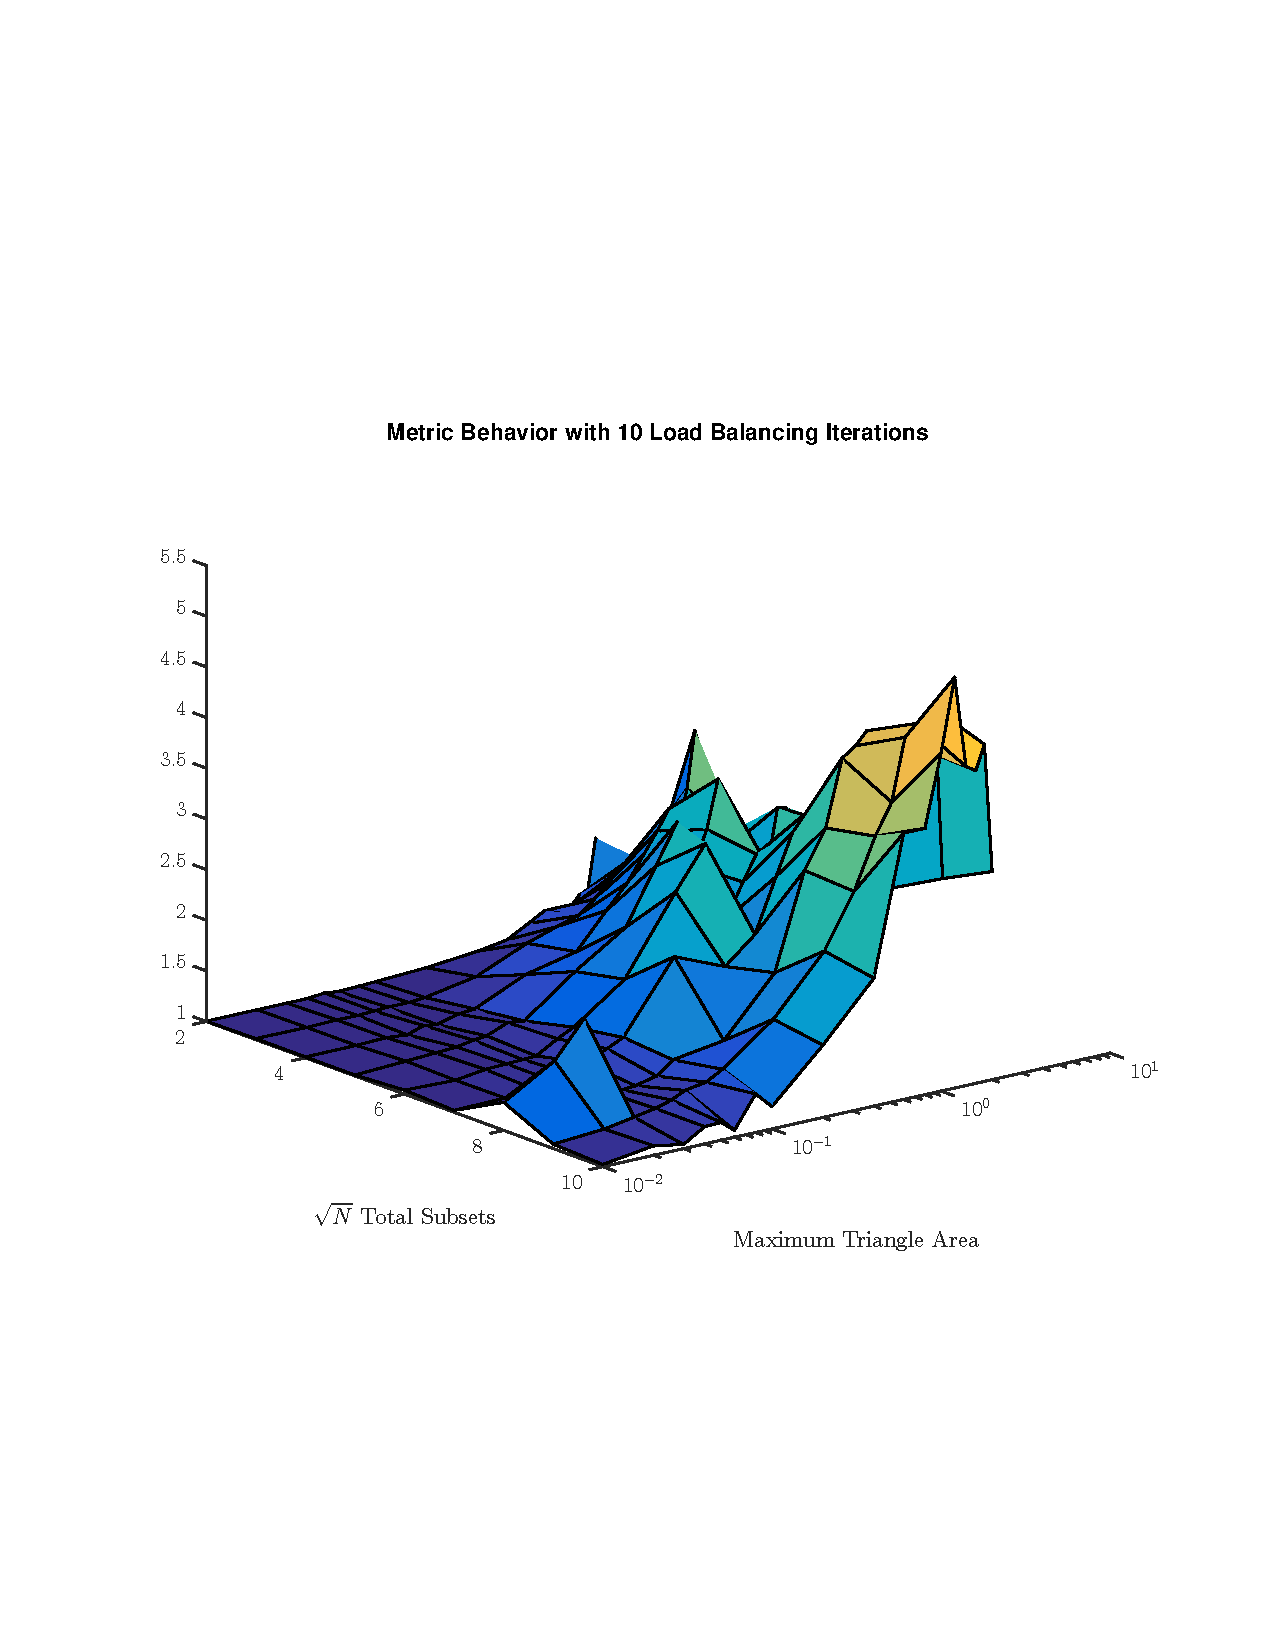
\includegraphics[width=85mm, trim = 0cm 5cm 0cm 5cm,clip]{figures/OppIter.pdf}
\caption{The metric behavior of the first test case run with 10 load balancing iterations.}
\label{oppiter}
\end{figure}

Figure \ref{samenoiter} shows the metric behavior for Fig. \ref{same}. The maximum metric is 22.6654 and occurs when Fig. \ref{same} is run with 8x8 subsets with a maximum triangle area of 1.8 cm\textsuperscript{2}. The minimum metric is 1.0024 and occurs when Fig. \ref{same} is run with 2x2 subsets with a maximum triangle are of 0.01 cm\textsuperscript{2}.

\begin{figure}
\centering
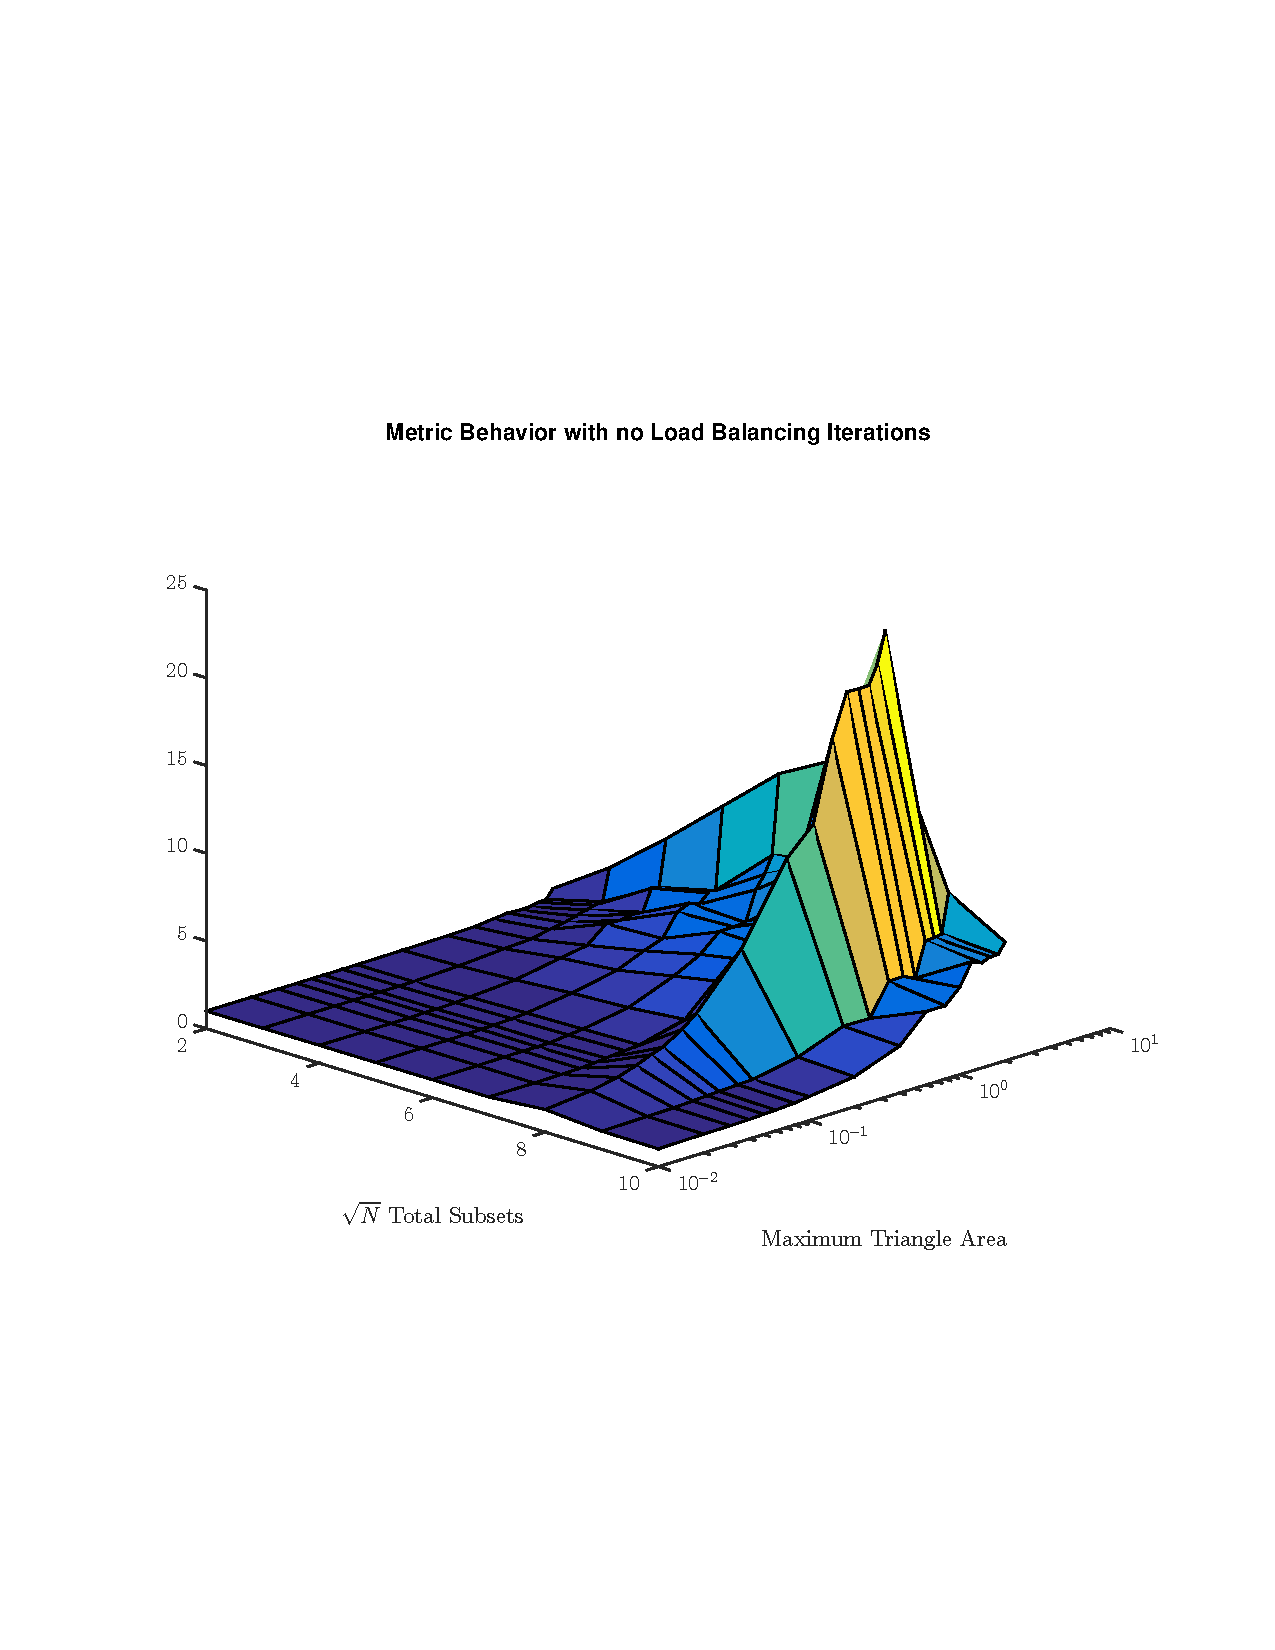
\includegraphics[width=85mm, trim = 2cm 5cm 0cm 5cm,clip]{figures/SameNoIter.pdf}
\caption{The metric behavior of the second test case run with no load balancing iterations.}
\label{samenoiter}
\end{figure}

Figure \ref{sameiter} shows the metric behavior for Fig. \ref{same} after ten load balancing iterations. The maximum metric is 3.9929 and occurs when Fig. \ref{same} is run with 10x10 subsets with a maximum triangle area of 1.8 cm\textsuperscript{2}. The minimum metric is 1.0024 and occurs when Fig. \ref{same} is run with 2x2 subsets with a maximum triangle are of 0.01 cm\textsuperscript{2}.

\begin{figure}
\centering
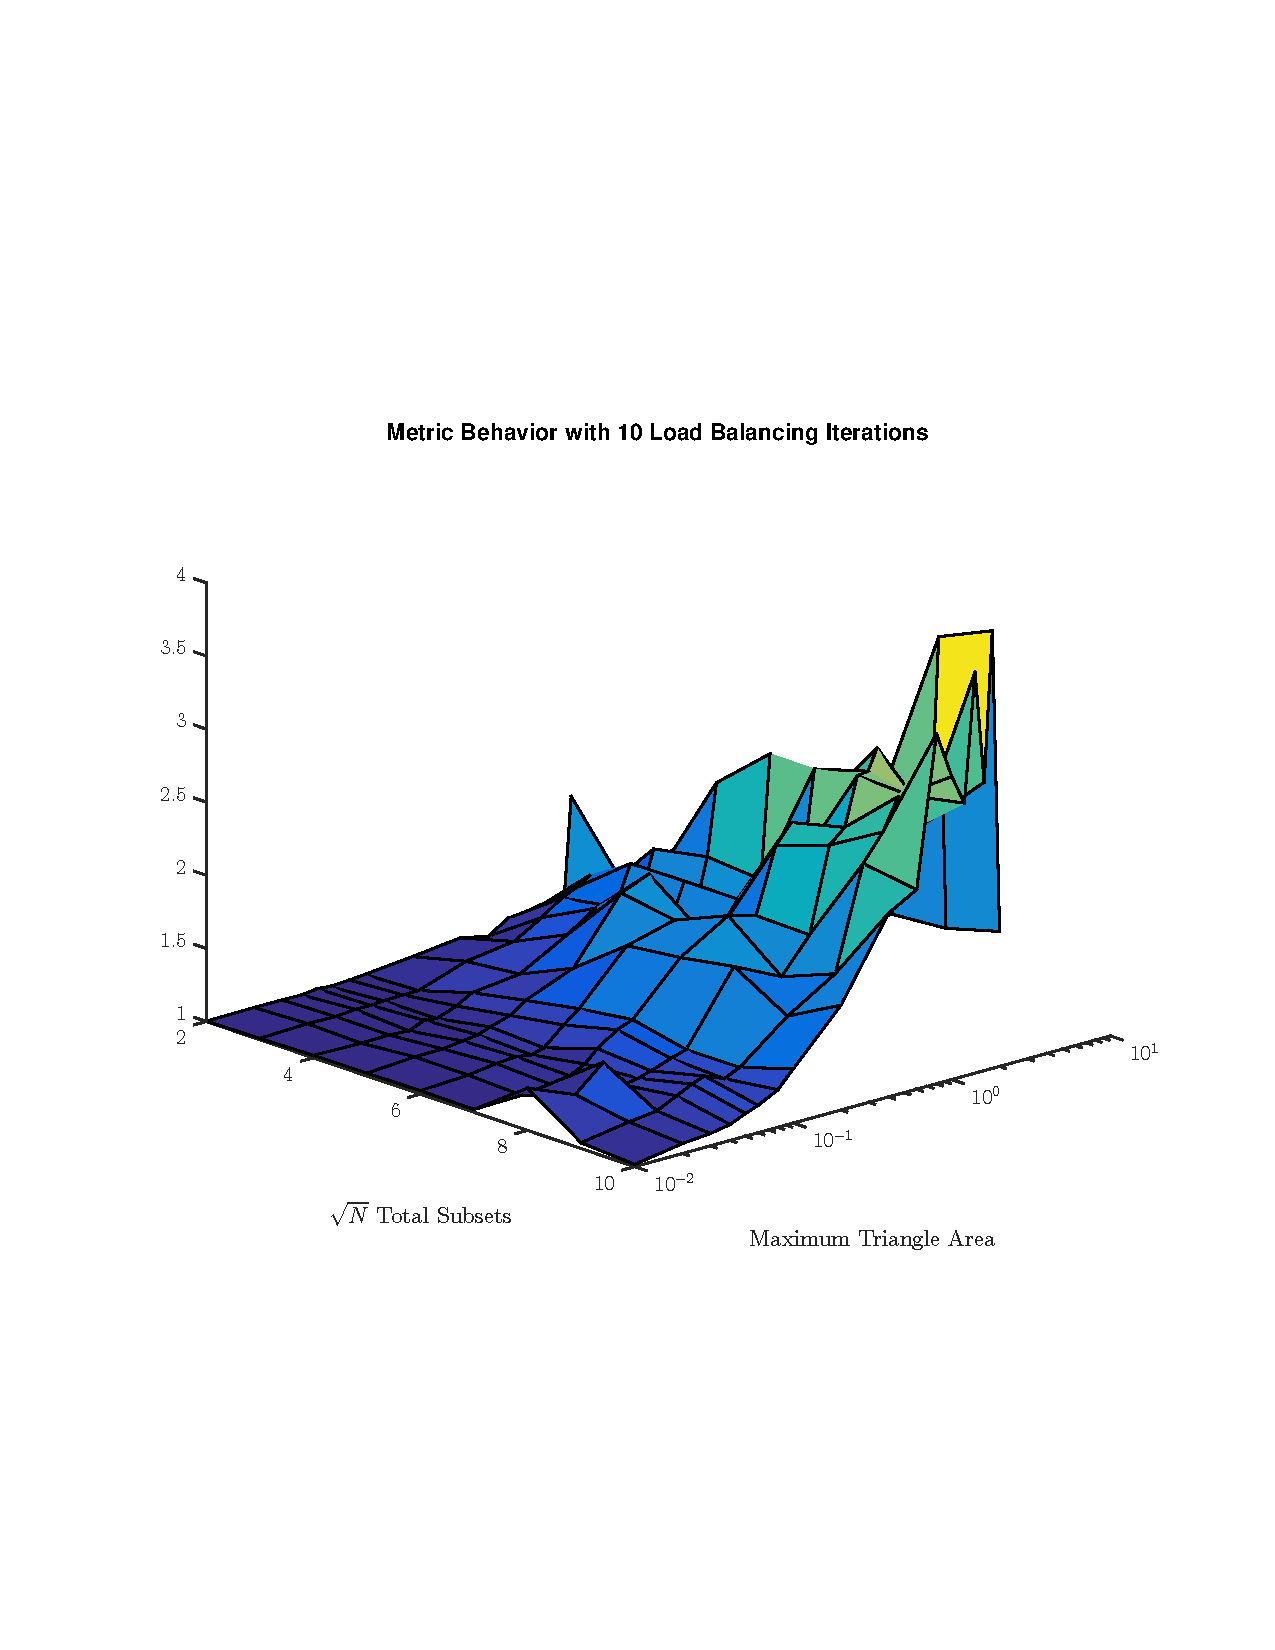
\includegraphics[width=85mm, trim = 2cm 5cm 0cm 5cm,clip]{figures/SameIter.pdf}
\caption{The metric behavior of the second test case run with 10 load balancing iterations.}
\label{sameiter}
\end{figure}

Figure \ref{latticenoiter} shows the metric behavior for Fig. \ref{lattice}. The maximum metric is 2.6489 and occurs when Fig. \ref{lattice} is run with 10x10 subsets with a maximum triangle area of 1.8 cm\textsuperscript{2}. The minimum metric is 1.0179 and occurs when Fig. \ref{lattice} is run with 2x2 subsets with a maximum triangle are of 0.08 cm\textsuperscript{2}.

\begin{figure}
\centering
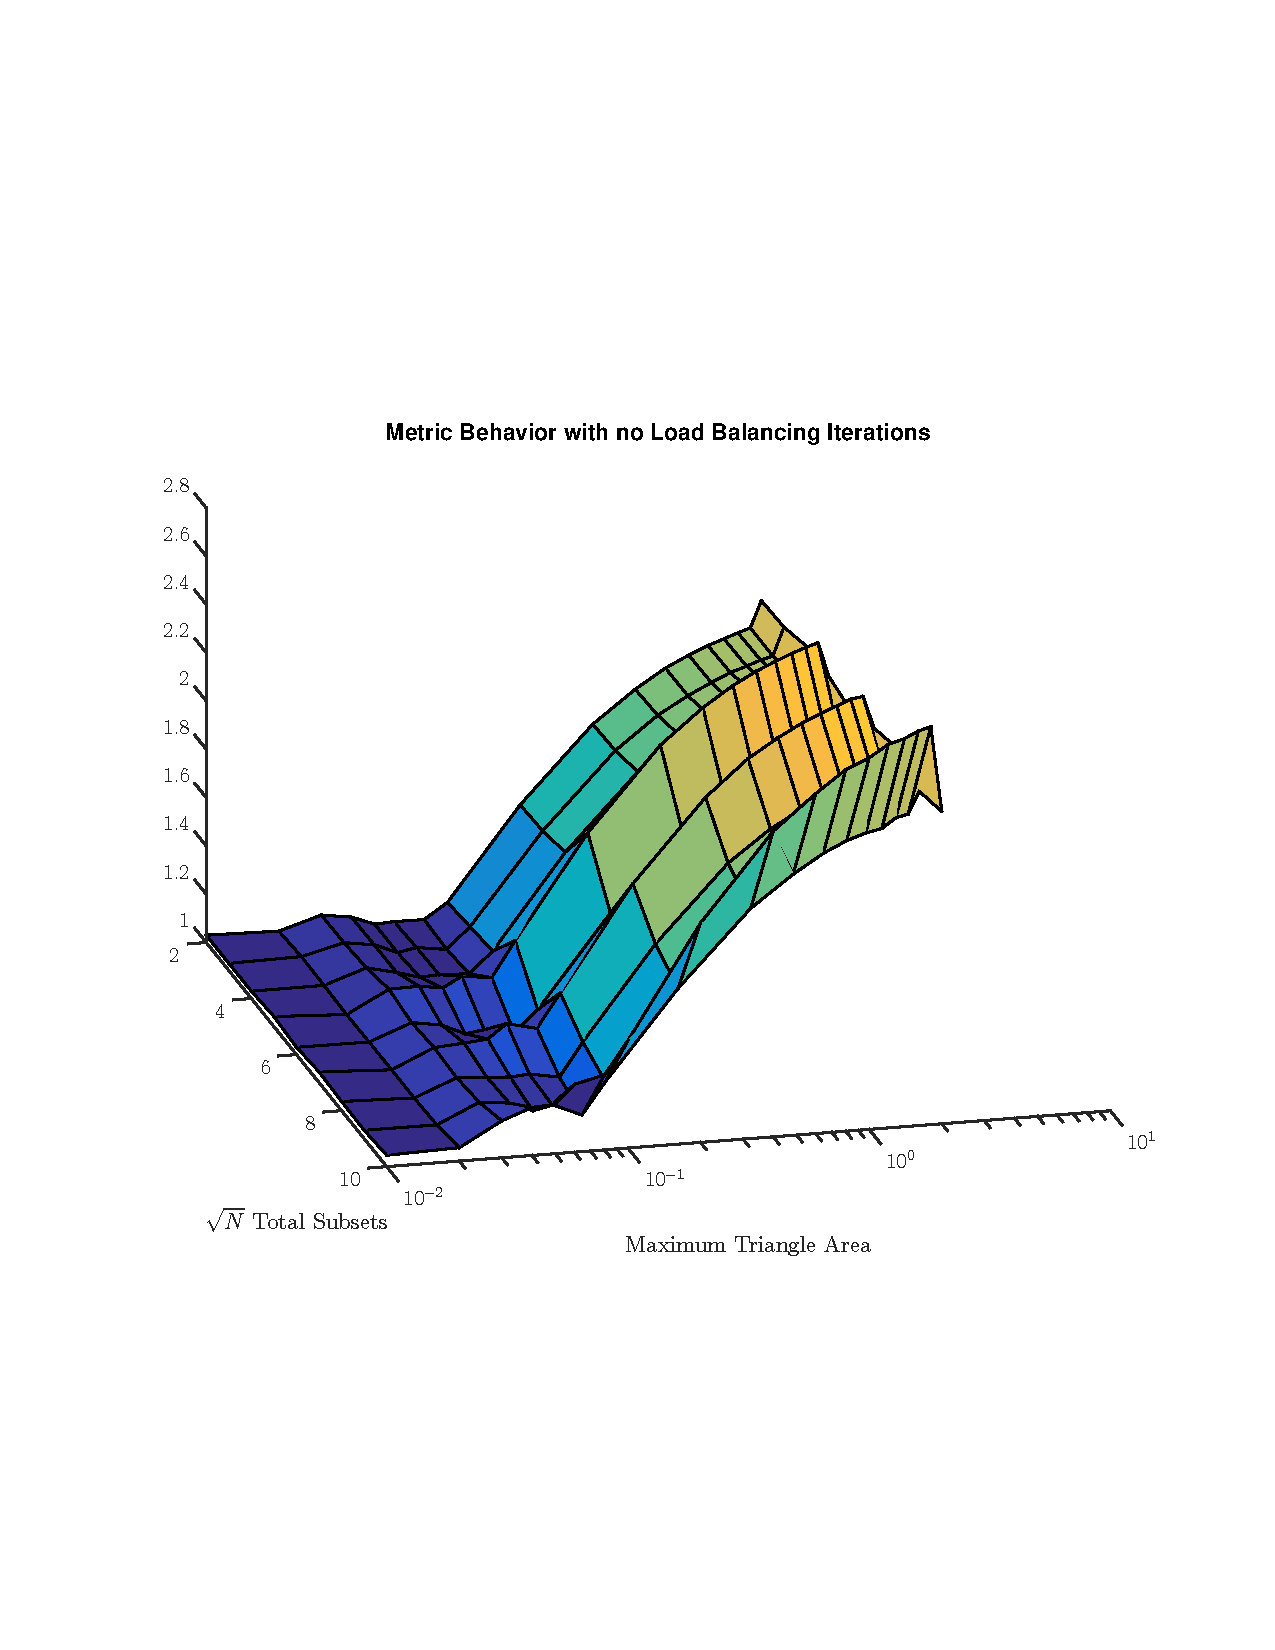
\includegraphics[width=85mm, trim = 0cm 5cm 0cm 5cm,clip]{figures/lattice_no_iter.pdf}
\caption{The difference in metric behavior of the third test case with no load balancing iterations.}
\label{latticenoiter}
\end{figure}

Figure \ref{latticeiter} shows the metric behavior for Fig. \ref{lattice} after ten load balancing iterations. The maximum metric is 2.2660 and occurs when Fig. \ref{lattice} is run with 10x10 subsets with a maximum triangle area of 0.4 cm\textsuperscript{2}. The minimum metric is 1.0021 and occurs when Fig. \ref{lattice} is run with 2x2 subsets with the Triangle's coarsest possible mesh.

\begin{figure}
\centering
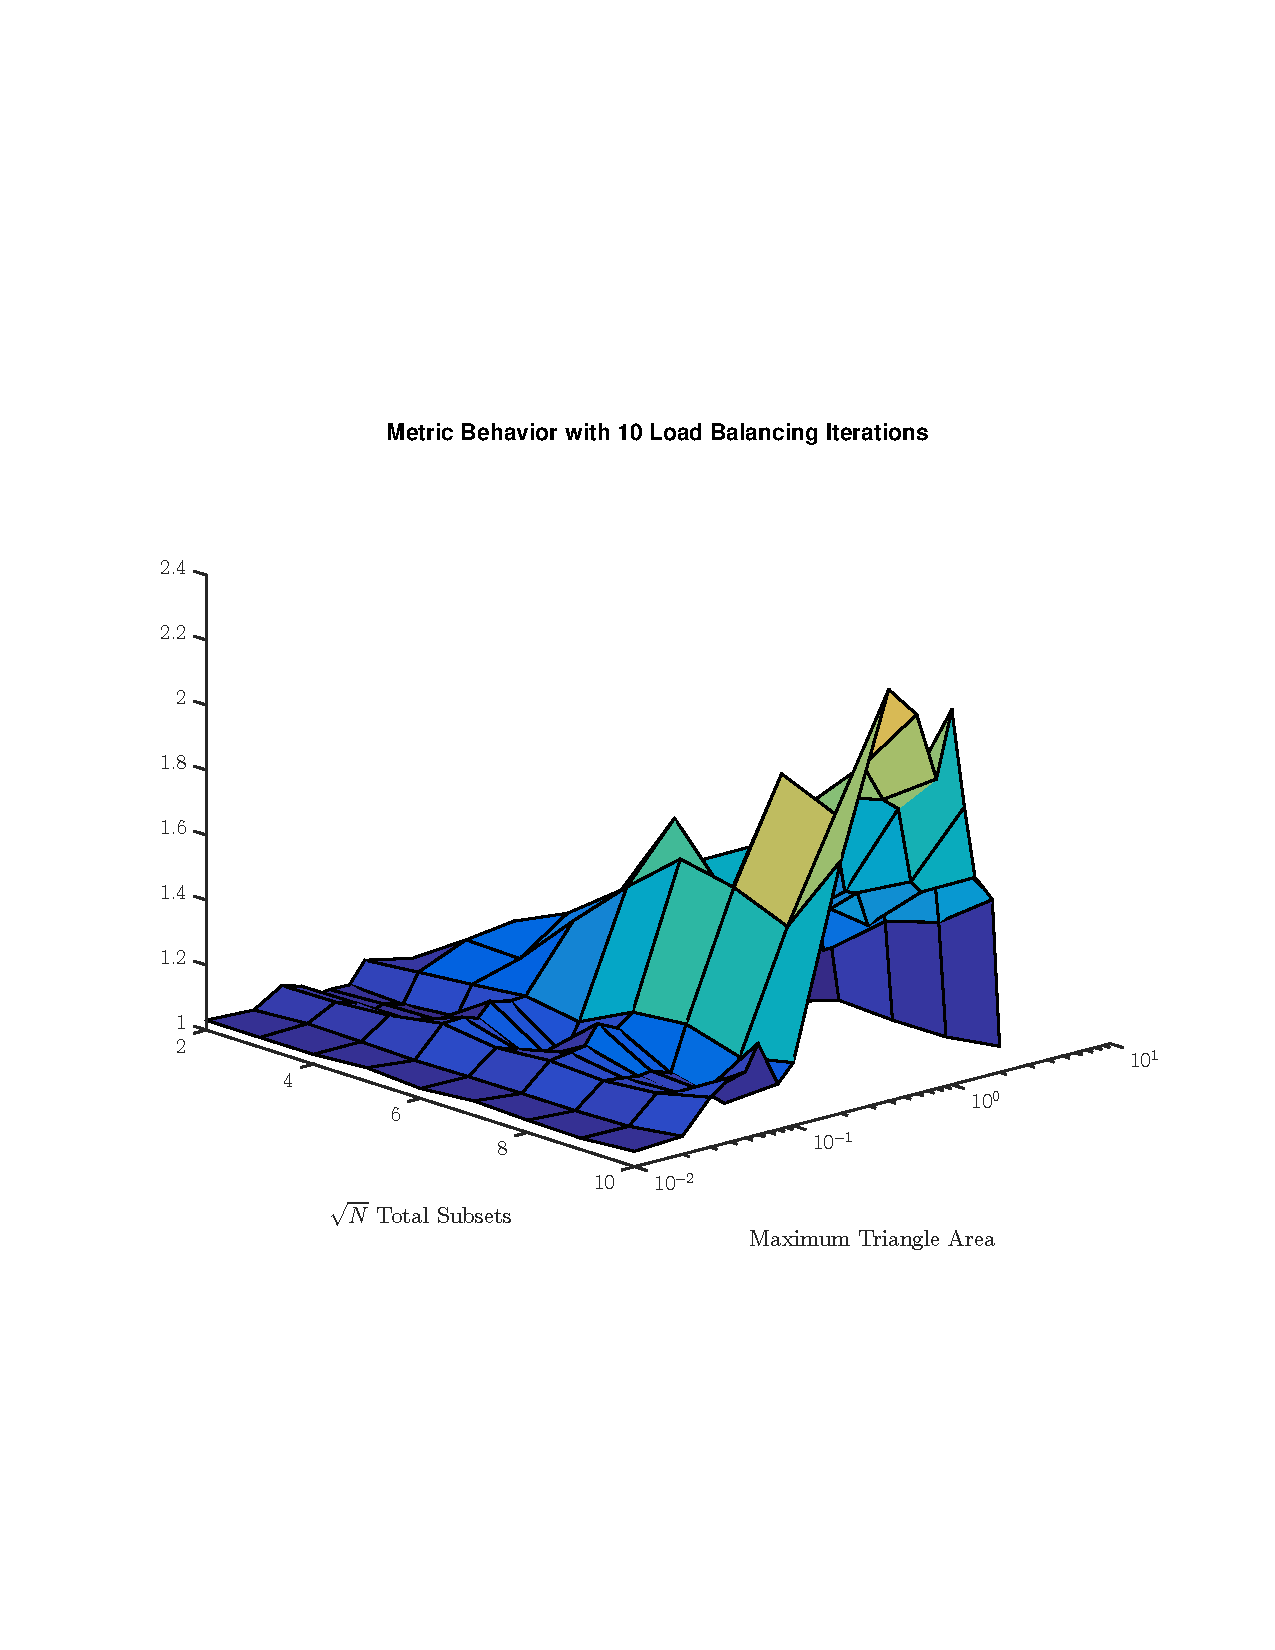
\includegraphics[width=85mm, trim = 0cm 5cm 0cm 5cm,clip]{figures/lattice_iter.pdf}
\caption{The difference in metric behavior of the third test case after ten load balancing iterations.}
\label{latticeiter}
\end{figure}

Because Fig. \ref{lattice} has more features and is more symmetric of a problem, the initial load balancing metric will not be as large as the load balancing metric of Figs. \ref{same} and \ref{opp}. As a result, the improvement in the load balancing metric after 10 iterations will not be as great in problems similar to Fig. \ref{lattice}. 

Good improvement is seen throughout all three test cases for all three inputs, particularly the first two test cases, which were initially very unbalanced. However, there were many inputs run that had problems with $f > 1.1$, which means many problems were unbalanced by more than 10\%. The user will not always have the luxury of choosing the number of subsets they want the problem run with, as this directly affects the number of processors the problem will be run with. Certain problems will require more processors and will require minimizing the total number of cells in the domain for the problem to complete running in a reasonable amount of time. As a result, improvements to the algorithm must be made. 

This can be done by changing how the cut lines are redistributed. Instead of changing entire row and column widths, the cut lines can be moved on the subset level. However, this can sacrifice the strict orthogonality that PDT currently utilizes to scale so well on a massively parallel scale\cite{mpadams2015}. Changes to the performance model and the scheduler would have to be made.

Another option is to implement domain overloading\cite{mpadams2015}, which is the logical extension of the work presented in this paper. This would involve processors owning different numbers of subsets, with no restriction on these subsets being contiguous. This would be the most effective method at perfecting this algorithm, and would lead to less problems being unbalanced by more than 10\%.

%%%%%%%%%%%%%%%%%%%%%%%%%%%%%%%%%%%%%%%%%%%%%%%%%%%%%%%%%%%%%%%%%%%%%%%%%%%%%%%%
\subsection{2D and 2D Extruded Meshing Capability}

To illustrate the newly implemented unstructured meshing capability in PDT, a neutron graphite experiment, modeled at Texas A\&M University as part of the DOE's NNSA PSAAP program, is used as an example. Figure~\ref{IM12D} shows the 2D mesh of the IM1 problem before and after 7 load-balancing iterations. The metric before any load balancing iterations is 42.15, and 2.99 after 7 iterations. The 3D extruded mesh is shown in Fig.~\ref{IM13D}.

%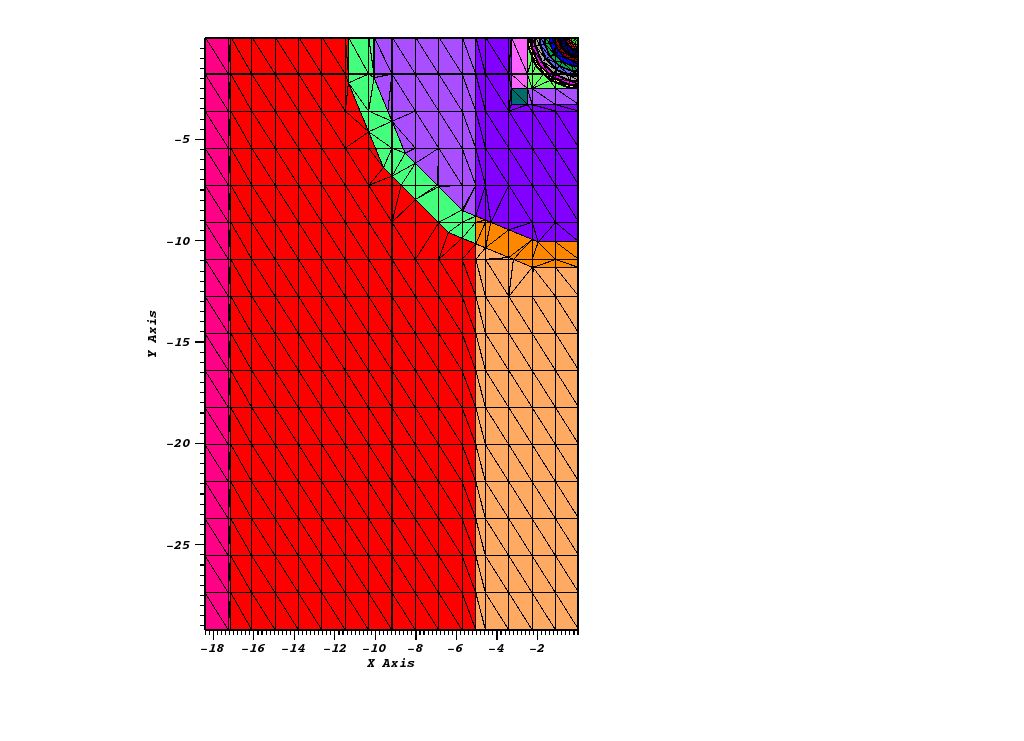
\includegraphics[scale=0.3]{figures/IM1_pre_iterations0000.png}
%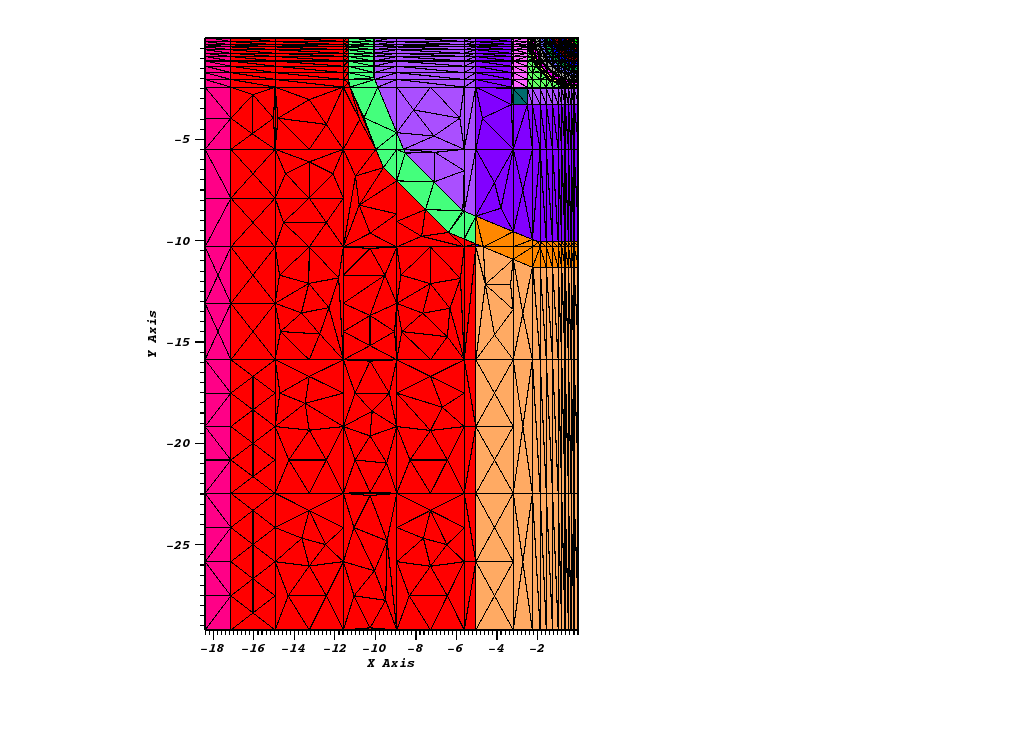
\includegraphics[scale=0.3]{figures/IM1_post_iterations0000.png}

\begin{figure}
\centering
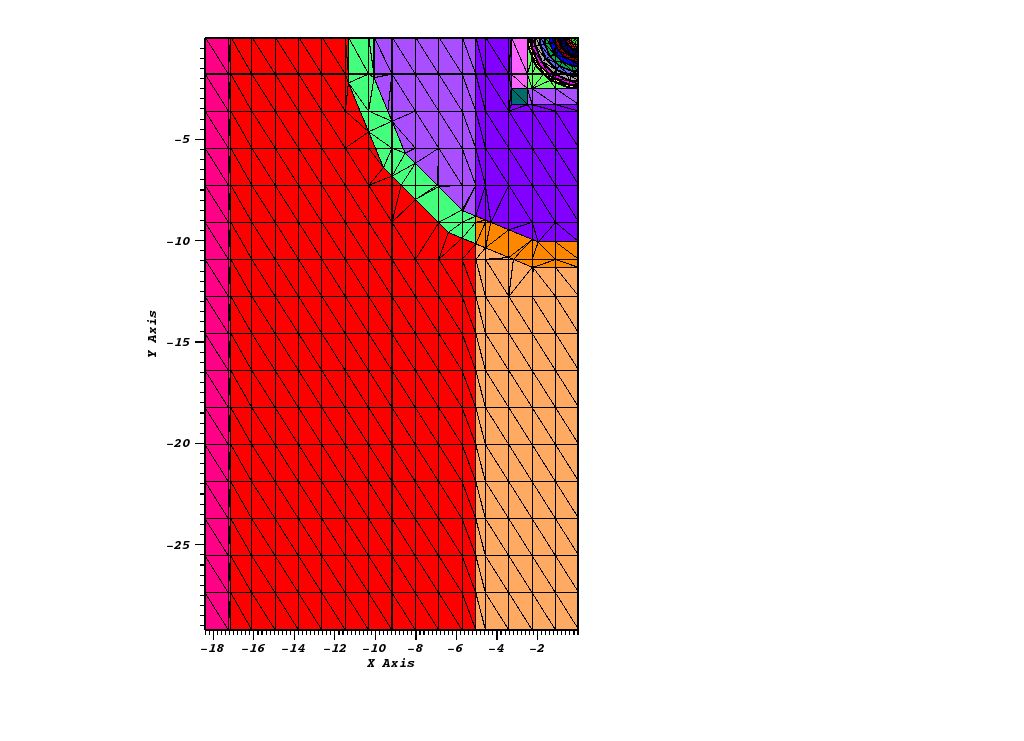
\includegraphics[width=85mm]{figures/IM1_pre_iterations0000.png}
\caption{The 2D mesh of the IM1 problem with no load balancing iterations.}
\label{IM12D}
\end{figure}

\begin{figure}
\centering
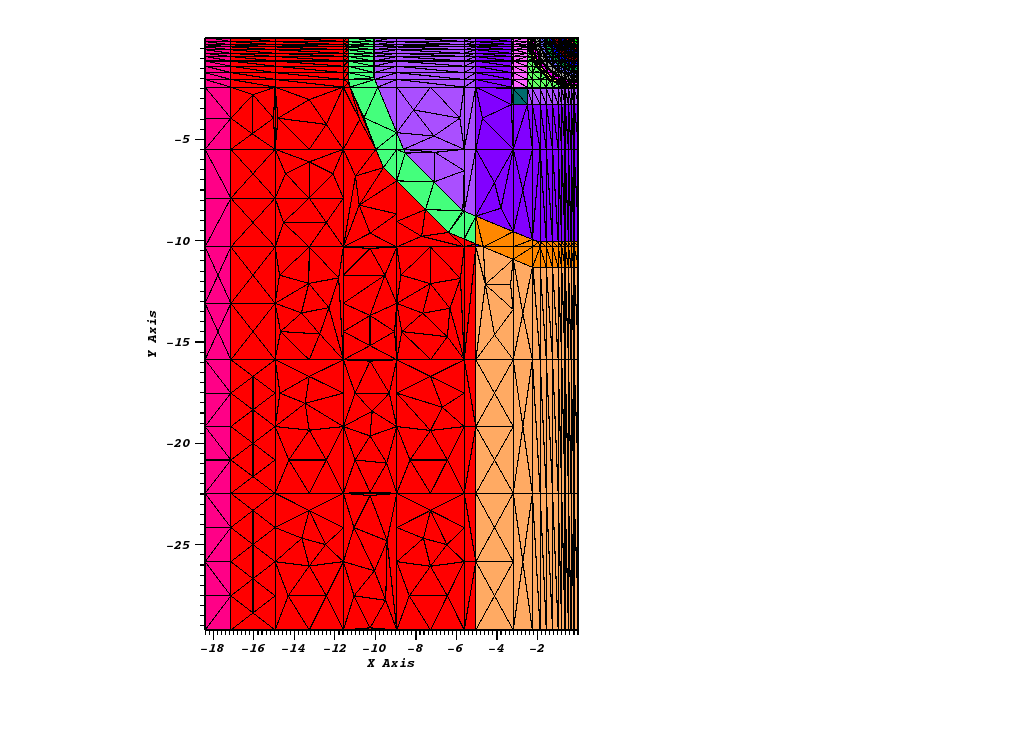
\includegraphics[width=85mm]{figures/IM1_post_iterations0000.png}
\caption{The 2D mesh of the IM1 problem with 7 load balancing iterations.}
\label{IM12D}
\end{figure}

\begin{figure}
\centering
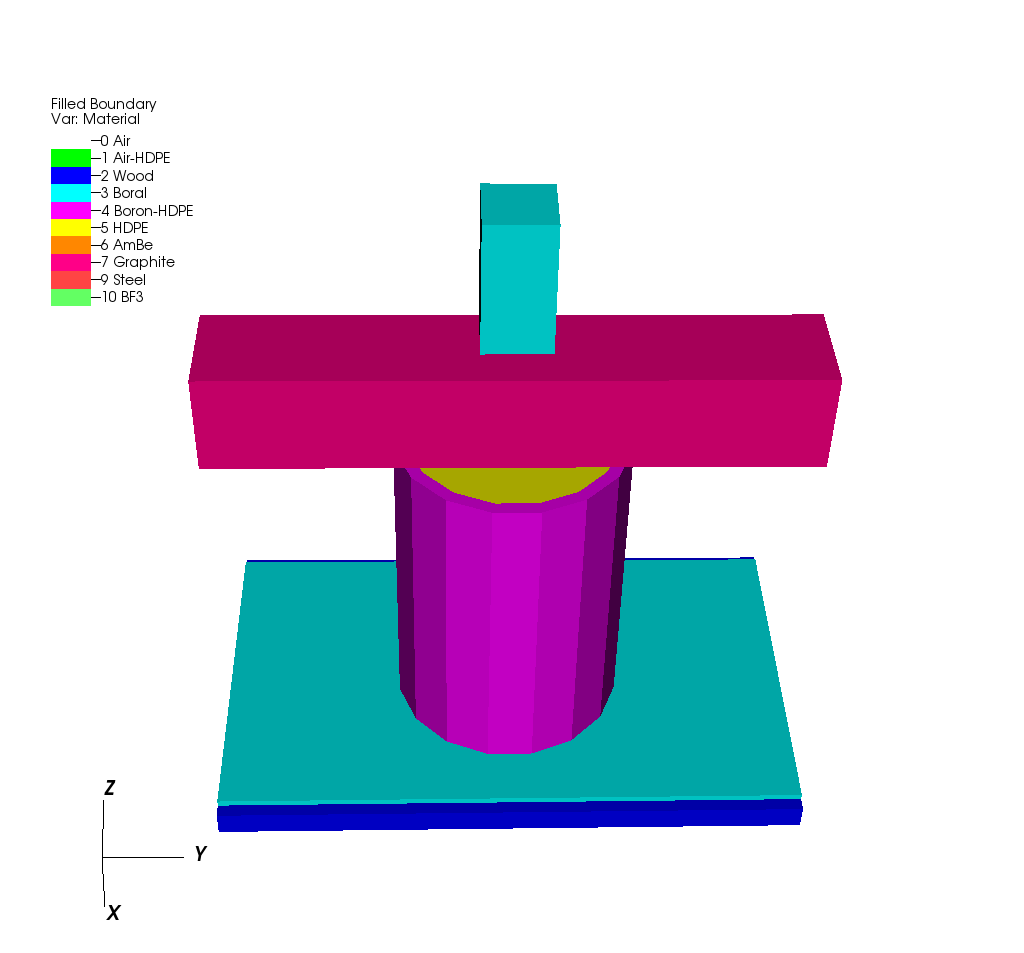
\includegraphics[width=85mm,trim= 0cm 0cm 0cm 3cm, clip]{figures/IM1_3D.png}
\caption{The 3D extruded view of the IM1 problem (HDPE cylinder with AmBe source; graphite block; detector and detector shroud).}
\label{IM13D}
\end{figure}


%%%%%%%%%%%%%%%%%%%%%%%%%%%%%%%%%%%%%%%%%%%%%%%%%%%%%%%%%%%%%%%%%%%%%%%%%%%%%%%%
\section{Conclusions}

In conclusion, the load balancing algorithm outlined in the Load Balancing Method section works well for more symmetric problems with a lot of features, and even works well for particularly unbalanced problems. As shown in the results, its effectiveness depends on the maximum triangle area used, and the number of subsets the user chooses to decompose the problem domain into. 

Good improvement is seen throughout all three test cases for all three inputs, particularly the first two test cases, which were initially very unbalanced. However, there were many inputs run that had problems with $f > 1.1$, which means many problems were unbalanced by more than 10\%. The user will not always have the luxury of choosing the number of subsets they want the problem run with, as this directly affects the number of processors the problem will be run with. Certain problems will require more processors and will require minimizing the total number of cells in the domain for the problem to complete running in a reasonable amount of time. As a result, improvements to the algorithm must be made. 

This can be done by changing how the cut lines are redistributed. Instead of changing entire row and column widths, the cut lines can be moved on the subset level. However, this can sacrifice the strict orthogonality that PDT currently utilizes to scale so well on a massively parallel scale\cite{mpadams2015}. Changes to the performance model and the scheduler would have to be made. This method is currently being implemented.

Another option is to implement domain overloading\cite{mpadams2015}, which is the logical extension of the work presented in this paper. This would involve processors owning different numbers of subsets, with no restriction on these subsets being contiguous. This would be the most effective method at perfecting this algorithm, and would lead to less problems being unbalanced by more than 10\%.

%%%%%%%%%%%%%%%%%%%%%%%%%%%%%%%%%%%%%%%%%%%%%%%%%%%%%%%%%%%%%%%%%%%%%%%%%%%%%%%%
%\appendix
%\section{Appendix}
%
%Numbering in the appendix is different:
%\begin{equation} \label{eq:appendix}
%  2 + 2 = 5\,.
%\end{equation}
%and another equation:
%\begin{equation} \label{eq:appendix2}
%  a + b = c\,.
%\end{equation}

%%%%%%%%%%%%%%%%%%%%%%%%%%%%%%%%%%%%%%%%%%%%%%%%%%%%%%%%%%%%%%%%%%%%%%%%%%%%%%%%
\section{Acknowledgments}
This material is based upon work supported by the Department of Energy, National Nuclear Security Administration, under Award Number(s) DE-NA0002376.

%%%%%%%%%%%%%%%%%%%%%%%%%%%%%%%%%%%%%%%%%%%%%%%%%%%%%%%%%%%%%%%%%%%%%%%%%%%%%%%%
\bibliographystyle{ans} % Don't forget to run BibTeX !
\bibliography{bibliography}

\end{document}

